\documentclass[fire,article,accept,oneauthor,pdftex]{Definitions/mdpi} 

% MDPI internal commands
\firstpage{1} 
\makeatletter 
\setcounter{page}{\@firstpage} 
\makeatother
\pubvolume{1}
\issuenum{1}
\articlenumber{0}
\pubyear{2026}
\copyrightyear{2026}
\externaleditor{Ioannis Gitas} 
\datereceived{9 February 2026} 
\daterevised{24 April 2026}
\dateaccepted{8 May 2026} 
\datepublished{ } 
%\hreflink{https://doi.org/} % If needed use \linebreak

% Additional packages
\usepackage{longtable}
\usepackage[utf8]{inputenc}

\usepackage{lmodern}

\newcommand{\degC}{$^\circ$C}

%=================================================================
% Full title of the paper (Capitalized)
\Title{Remote Sensing in Rangeland Fire Ecology: Comparing Imagery to Measured Fire Behavior and Burn Severity Across Prescribed Burns and Wildfires}%EE: Attention: title altered

% MDPI internal command: Title for citation in the left column
%\TitleCitation{Remote sensing in rangeland fire ecology}

\newcommand{\orcidauthorA}{0000-0002-3763-7641} 

% Authors, for the paper (add full first names)
\Author{Devan Allen McGranahan %MDPI: 1. Please carefully check the accuracy of names and affiliations. Author: Names and affiliation accurate.
%2. We removed aff. number since there is only one affiliation. Please confirm. 
% 3. Please confirm if the first-note need to be retained or can be removed.
%MDPI: Important information: once the paper is accepted, we will not accept any changes on the Authorship, affiliations, data, contents, Acknowledgments, funding, etc. So please carefully check your paper.
%1. The initial layout for your manuscript was done by our layout team. Please do not change the layout of main text as well as references, otherwise we cannot proceed to the next step.
%2. Please do not delete our comments.
%3. Please revise and answer all questions that we proposed, such as: “It should be italic”; “I confirm”; “I have checked and revised all.”
%4. Please directly correct on this version.
%5. Please make sure that all the symbols in the paper are of the same format.
%6. Please make sure the first citation of each reference is mentioned in numerical order.
 $^{\dagger}$\orcidA{} }


% MDPI internal command: Authors, for metadata in PDF
\AuthorNames{Devan Allen McGranahan}

% Affiliations / Addresses (Add [1] after \address if there is only one affiliation.)
\address[1]{%
Livestock \& Range Research Laboratory, Agricultural Research Service, USDA, %MDPI: We arranged the authors’ address information from subordinate to superior. Please check and confirm this modification.
 Miles City, MT 59301, USA; devan.mcgranahan@usda.gov %MDPI: Capitalized email address is not recommended; we changed it to lowercase. Please confirm. Author: OK
}

\firstnote{\hangafter=1 \hangindent=1.05em \hspace{-0.82em}The US Department of Agriculture is an equal opportunity lender, provider, and employer.}


% Abstract (Do not use inserted blank lines, i.e. \\)
\abstract{Wildland fire scientists have made substantial advances in measuring fire behavior, but properly collecting data is often beyond the capacity of prescribed fire managers and by definition all but impossible for wildfire events. 
	While a method for the immediate assessment of burn severity has been developed around multispectral imagery from space-based Earth observation systems, there has been little comparison of these post hoc metrics to actual fire behavior.
	Meanwhile, the application of research results from experimental prescribed burns to rangeland affected by wildfire can be impeded by a lack of understanding of how immediate burn severity  differs between wildfires and prescribed burns, especially in rangelands. 
	Overall, much of what is known about wildland fire behavior, severity, and effects comes from forests, whereas rangelands are characterized by having lower fuel loads comprised of fine vegetation that promotes high rates of spread and brief residence time. 
	This paper provides rangeland-specific information on the relationships between direct field-based fire behavior measurements and a space-based index of burn severity (differenced Normalized Burn Ratio, $\Delta$NBR, from Sentinel-2 imagery), and uses those data to compare burn severity across 54 prescribed burns in North Dakota, USA, and 28 nearby wildfires in the US Northern Great Plains.
 	In prescribed burns, remotely sensed burn severity increased with rate of spread and flame temperature 15 cm above the ground, but had no statistically significant relationship with soil surface temperature. 
 	In the semi-arid western zone of the Northern Great Plains, wildfires and prescribed burns had similar, low--moderate severity; wildfires in the eastern zone tended to be of moderately high severity and thus greater than the low severity of the experimental prescribed burns. 
	 By describing meaningful gradients in surface fire behavior in rangelands with $\Delta$NBR, even those without the capacity to measure fire behavior in the field can monitor prescribed fire effectiveness and incorporate burn severity in adaptive management plans. 
	Understanding the relationship between burn severity across wildfires and prescribed burns is a critical step in applying knowledge gained from research on prescribed fires to areas impacted by wildfire. 
	Resistance to prescribed burning might be overcome by increasing livestock managers' experience with post-fire forage resources through grazing areas burned in unintentional wildfires, but current practice and policy discourage or outright prevent ranchers from doing so.
	Future research ought to connect burn severity with ecosystem recovery metrics to ensure post-fire grazing does not impair rangeland sustainability. \vspace{36pt}}

% Keywords
\keyword{differenced %MDPI: 1. We removed the uppercase in Keywords. Please confirm the revision. % Author: OK
% 2. We changed `Delta' to symbol, please confirm.  Author: OK
 Normalized Burn Ratio ($\Delta$NBR); rangeland fire ecology and %MDPI: Please check whether this ``and'' should be revised to semi-colon to separate keyword. Author: 'and' is currect.
 \linebreak management; rate of spread; thermocouple dataloggers; US Northern Great Plains;\linebreak wildland fire behavior }

\begin{document}

\section{Introduction}

Both in-field measurements of fire behavior and satellite-based Earth observation systems are available for the description of variability in several aspects of the wildland fire environment, but few direct comparisons between data derived from remotely sensed products and in-field sensors have been presented. 
Such a novel comparison is particularly useful in rangeland ecosystems, where the lack of forest canopy might allow managers and others unable to collect in-field fire behavior measurements to still describe variability using remotely sensed products.  

Wildland fire scientists use the term \emph{fire behavior}%MDPI: Please confirm if the italics is unnecessary and can be removed. The following highlights are the same. Author: The italics are correct, do not remove.
 to describe energy release by the combustion of vegetation in terms of how fast fire moves, how much heat is released, and how long burning lasts \cite{mcgranahan2021a, finney2021}. 
Some of these are immediately observable---one can measure rate of spread simply by timing the passage of a flame front between points of a known distance apart; the length of a flame is related to energy release \cite{rothermel1980}. 
But each of these metrics requires direct observation of the flame front, which is often precluded by smoke, lack of access, or the general danger to personnel posed by fire moving freely about. 
And while post-burn observations such as scorch height on trees can be used to infer intensity after the fact \cite{rothermel1980}, such methods have limited value in the rangeland ecosystems that cover approximately 54\% of the Earth's terrestrial surface and are characterized by having few if any trees \cite{ilri2021}. 

\subsection{Direct Measurements of Fire Behavior} 

Several methods directly measure fire behavior beyond human line of sight. 
As a prominent property of fire is heat, wildland fire scientists have long tried to measure fire behavior in terms of temperature.
For at least 75 years, measuring temperature in wildland fires has predominantly relied upon \emph{thermocouples}---pairs of two wires, composed of different metals, each of which transmit slightly different electric signals when their shared junction is heated; at the other end of the cable, differences in electrical properties across the two wires can be detected and converted to temperature \cite{vaartaja1949, engle1989,mcgranahan2020a, pavlasek2015, shannon2003}. 

Despite their ubiquity in wildland fire research, thermocouple systems have substantial limitations. 
Firstly, the physical limitations, \emph{e.g.,} %MDPI: We removed the italics. Please confirm this revision. Same to i.e. Author: Do not remove the italics for Latin abbreviations.
 response lags as the thermocouple material itself gains and loses heat from the material with which it is in contact, and  underestimations due to the fact that the junction is losing heat to the ambient environment as well as absorbing it \cite{walker1968,lemaire2017}.  These errors are greatest when the temperature discrepancy between the junction and the media is greatest \cite{blevins1999}, which is exactly when flame fronts arrive at the sensor.
Finally, the junction retains heat even after the flame front passes and continues to register elevated temperatures; this post-frontal %EE: Please check that intended meaning was retained.  Author: meaning was not retained. Original correct text restored.
period is often erroneously interpreted as ``residual heating'' even when the media the junction is in contact with has returned to ambient temperature \cite{mcgranahan2020a}. 


Secondly, even accurately measured temperature is a poor metric of fire behavior. 
Sensor placement has an outsized impact on temperature readings: the temperature of a single flame varies with distance from its base, and the vertical distribution of fuel can effect differences in the heating profile as great as whether temperatures increase or decrease with height away from the ground. 
Furthermore, recent work has called into question the decades-old concept that organisms have specific temperature mortality thresholds~\mbox{\cite{smith2016, pingree2019}}; better is to quantify the total exposure of tissue to heat energy over time \cite{wright1970, dickinson2004, bova2005}.
Thus, Alexander (\cite{alexander1982}, p. 350) concluded, ``Measuring temperature merely introduces a cumbersome, secondary step in the study of fire effects when direct linkage to one or more fire-behavior characteristics would be more profitable,'' and Bova and Dickinson~\cite{bova2008} urge fire ecologists to move ``beyond fire temperatures.''

For many wildland fire scientists, rate of spread has become the most reliable metric of fire behavior---conceptually simple; relatively easy to observe, measure, and report; and a step towards calculating intensity, as an input in the Byram equation \cite{byram1959}. 
Rate of spread is not perfect---it is affected by each component of the fire triangle but not singularly attributable to any, meaning several combinations of variables in the wildland fire environment can produce the same rate of spread \cite{finney2021}. 
But rate of spread is a common output in fire behavior prediction models \cite{perry1998, cruz2018}, particularly of head fires spreading with the wind. 
While such one-dimensional rate of spread is theoretically relatively easy to measure, especially during prescribed burns---stakes can be pre-positioned and a stopwatch used to time flame front travel between them---in reality, these measurements are challenged first by needing to ensure stakes are positioned perpendicular to the flame front, and second by needing to be within visual contact of the fuelbed ahead of the advancing fire.

Alternatively, measuring fire spread through a two-dimensional array of sensors has two advantages: it can be calculated regardless of the direction of spread, and does not need a human present \cite{finney2021}.
Thermocouple dataloggers can be used, but with the twist that the information of most value is the timestamp recorded when the flame front hits each sensor in the array: trigonometry can be applied to these arrival times to calculate the average speed at which the flame front moved through the array \cite{simard1982, simard1984, clements2019, mcgranahan2021, mcgranahan2023} (Figure \ref{Fig:FeatherFlame}). 


\begin{figure}[H]
	\centering
	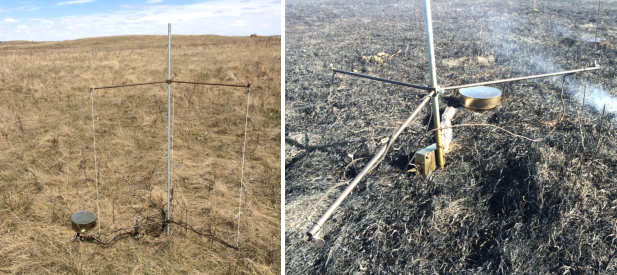
\includegraphics[width=0.98\columnwidth]{FeatherFlame.pdf}
	\caption{The %MDPI: 1. We moved figure after its 1st citation and revised ref. citation in order. Please confirm. Author: OK
	%2. Please note that the size of figures will be adjusted appropriately to ensure the clarity and readability of the image. Changes to the position of figures and tables may occur during the production stage. 
	%3. Please ensure that permission has been obtained and there is no copyright issue. If copyright is needed, please provide a citation in the following format: “Reprinted/adapted with permission from Ref. [XX]. Copyright year, copyright owner’s name”. More details on “Copyright and Licensing” are available via the following link: https://www.mdpi.com/ethics#10. Please confirm this for all figures and tables. Author: No copyright issue.
 FeatherFlame is an example of a thermocouple-based system designed to measure two-dimensional rate of spread, shown here deployed before a prescribed fire (\textbf{left}) and after the fire had passed (\textbf{right}). 
		The 1 m equilateral triangle holds three K-type thermocouples 15 cm above the soil surface. 
		Using the timestamps associated with flame temperatures recorded by the Arduino-based datalogger allows calculation of rate of spread through the array. 
		A fourth thermocouple is placed under litter at the soil surface. 
		The cylindrical galvanized cap protects the datalogger from heat, allowing \emph{in agris} %MDPI: Please confirm if the italics is unnecessary and can be removed. The following highlights are the same. Author: Italics are correct and should not be removed.
fire behavior measurements.
	The system on the left is shown deployed with optional passive flame height sensors following \cite{finney1992}.   }
	\label{Fig:FeatherFlame} % Fig.~\ref{Fig:FeatherFlame}
\end{figure}

\subsection{Remote Sensing in Fire Ecology} 

Beyond field-based measurements, space-based Earth observation systems are increasingly being applied in wildland fire science \cite{szpakowski2019}. 
Fire ecologists have made particular use of the Normalized Burn Ratio (NBR), a multispectral product derived from Near-Infrared and Shortwave Infrared wavelengths, which have specific responses to reflectance changes caused by burning \cite{key2006a}. 
Changes effected by a specific fire event can be isolated by subtracting, or \emph{differencing}, post-fire NBR values from NBR values of the same point prior to the fire, creating a metric called Differenced Normalized Burn Ratio ($\Delta$NBR; Figure~\ref{Fig:NBRexample}). 

\vspace{-9pt}
\begin{figure}[H]
%	\centering
	%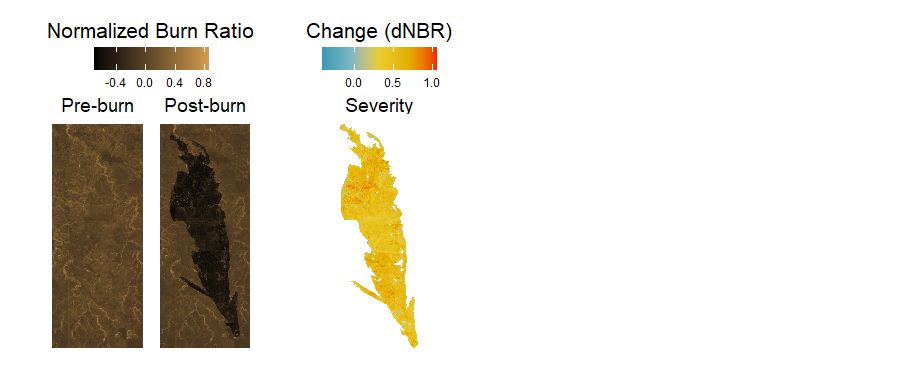
\includegraphics[width=1\columnwidth, trim={30 30 340 15},clip]	{example_wide.png} % left bottom right top
	
\includegraphics[width=0.7\columnwidth, trim={10 0 0 0},clip]{nbr_gg.png}~
	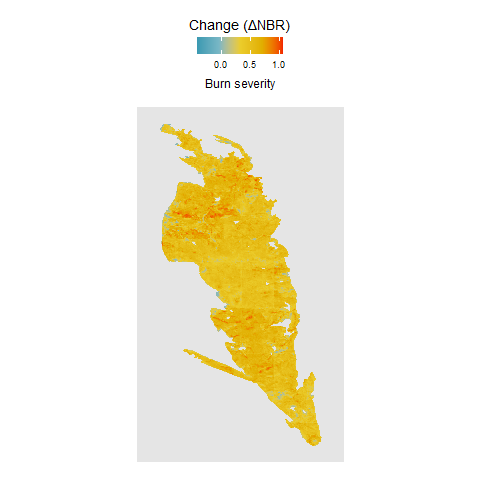
\includegraphics[width=0.27\columnwidth, trim={150 0 150 0},clip]{dnbr_gg.png}

	\caption{An %MDPI: We revised hyphen into minus sign in the figure. Please confirm. Author: OK
 example of a wildland fire from multipsectral imagery; 	see Figure~\ref{Fig:TrueColor} for true color imagery, including a capture of the fire while it was burning.
		The longest axis of this fire extended 12~km (7.5 miles).
				(\textbf{Left}) %MDPI: We revised italic into bold according to our rules. Please confirm the format revision. Same to the following. Author: OK
 The Normalized Burn Ratio for before and after scenes from a fire in North Dakota, derived from Sentinel-2 Near-Infrared and Shortwave Infrared sensors.
		(\textbf{Right}) Burn severity is calculated as the difference between the before and after NBR (Differenced NBR, or $\Delta$NBR), a measure of how much aboveground material the fire removed via combustion.
 }
	\label{Fig:NBRexample} % Fig.~\ref{Fig:NBRexample}
\end{figure}

Fire ecologists use $\Delta$NBR to estimate burn severity, defined in the context of interpreting remotely sensed products as ``the degree of environmental change caused by fire~(\mbox{\cite{key2006a}, p. LA-6}).''
Temporal scale is a very important factor in the definition and interpretation of a $\Delta$NBR value. 
Generally speaking, burn severity assessments can be divided into \emph{extended} and \emph{immediate} \cite{key2006a,veraverbeke2010}.
The Monitoring Trends in Burn Severity program uses both imagery from immediately after a fire, to assess first-order effects on soil and vegetation consumption, and from the next growing season, to identify overall mortality to tree canopies in forests \cite{eidenshink2007a}.
The temporal distinction is particularly important in grasslands, where fire might remove all aboveground plant biomass down to mineral soil---by most definitions, high severity in an immediate assessment---but herbaceous plants have typically regrown by the end of the next growing season, which an extended assessment would classify as low severity \cite{lentile2006}. 

\subsection{Fire Management in the 21st %MDPI: We removed the superscript. Please confirm. Same to the following `th'. Author: OK
 Century}
	
European colonization altered fire regimes around the world through top--down, command-and-control management that viewed wildland fire as destructive---and ironically, might have exacerbated the issue. 
As in many European and post-European nations, the United States had tight control over wildland fire by the middle of the 20th century by suppressing unintentional ignitions and excluding intentional ignitions, especially cultural burning \cite{mcgranahan2021a, donovan2007}. 
But several ecosystems have been diagnosed with fire deficits in which the decades-long elimination of fire has had negative ecological effects and led to a buildup of vegetation biomass that drives high-intensity fires that are often uncharacteristically severe and difficult to control \cite{parks2015,kolden2019}. 
Management interventions often focus on fuel reduction through mechanical thinning or prescribed burning; conducted under less extreme conditions than wildfires typically occur, these ``good'' fires consume hazardous fuels without effecting high severity to the rest of the ecosystem, and have shown varying degrees of effectiveness in reducing the severity of subsequent wildfires \cite{fernandes2003, brodie2024}. 

\subsection{Objectives and Hypotheses} 

The intent of this paper is two-fold: to provide rangeland-specific information on the relationships between direct field-based fire behavior measurements and space-based measurements of burn severity, and use those data to compare burn severity across prescribed burns and wildfires. 
Connecting remotely sensed data to direct measurements helps calibrate assessments and monitoring programs that are unable to collect field-based fire behavior data but want insight into whether variation in remotely sensed products has a meaningful relationship with ecological processes on the ground. 
Understanding how burn severity differs between prescribed burns and wildfires informs the transferability of ecological data on fire effects from burning experiments to broader landscapes affected by wildfire.
This paper draws on prescribed burns and wildfires in the semi-arid Northwestern Great Plains of eastern Montana and western North Dakota, USA, and the mesic mixed-grass prairies of central North Dakota.

The specific hypotheses tested here include: 
\begin{enumerate}[leftmargin=*,labelsep=4.9mm] 
	\item A positive linear relationship between field-based fire behavior and space-based burn severity metrics, as higher-intensity fires remove more aboveground plant material and expose more of the mineral surface to satellites.
	\item No difference in burn severity among wildfires and prescribed burns, as prescribed burns have been shown to demonstrate a wide range of burn severity that likely overlaps with that of wildfires (e.g., \cite{mcgranahan2025}). 
\end{enumerate}

 
\section{Methods %MDPI: This is a reminder: 
%Please check the whole paper and ensure:
%1. All software used in this paper have been stated the version number.
%2. All equipment used in this paper have been stated the name of the manufacturer/company, city, abbreviated state name (USA or Canadian companies), and country from where they were sourced. Author: OK
} 

\subsection{Study Area}

The primary geographical scope of this study is the Northern Great Plains of the United States, specifically two experimental research locations in south-central and southwestern North Dakota (Figure~\ref{Fig:StudyMap}). 
The south-central research location, referred to hereafter as the eastern location and in the eastern zone, is the North Dakota State University Central Grasslands Research Extension Center near Streeter, ND, located within the Northwestern Glaciated Plains in a relatively humid, mixed-grass prairie pothole landscape known as the Missouri Coteau. 

The southwestern research location, referred to hereafter as the western location and in the western zone, is focused around the North Dakota State University Hettinger Research Extension Center in Hettinger, ND, located within the semi-arid mixed-grass prairie of the Northwestern Great Plains. 
Research activities at the western location were conducted by North Dakota State University personnel on two blocks of Center-managed rangeland pastures within 5 km of the Center and another privately owned ranch approximately 20~km to the east of Hettinger.

\begin{figure}[H]
%	\centering
	
\includegraphics[width=0.99\textwidth]{study_map-1.pdf}
	\caption{Location %MDPI: Please confirm if the black-line area/red and green colors/etc. need extra explanations. If so, please add. Author: All is OK
 of rangeland research areas with experimental prescribed burns ($R_{X}$) and comparison wildfires ($\times$, $+$) in the Northern Great Plains (green icons indicate eastern zone, brown indicates western). 
		Precipitation anomaly refers to the difference from mean annual precipitation at each of the western and eastern research locations for the study period (2017--2024); gray shaded areas have precipitation anomalies that exceed $\pm$ 3 standard deviations of mean annual precipitation and thus wildfires from these areas were excluded.
		Eastern and western zones align loosely with EPA Level III ecoregions NW Glaciated Plains and NW Great Plains, respectively (Figure~\ref{AppFig:RegionMap}), with the exception of five wildfires near the Missouri River in south-central North Dakota being assigned to the eastern zone, which has substantially fewer wildfires than the western zone for comparison. 
		Inset: Study region within broader US Great Plains and continental US. }
	\label{Fig:StudyMap} %Fig.~\ref{Fig:StudyMap}
\end{figure}

\subsection{Data Sources} 

This study reports on both prescribed burns conducted as part of rangeland ecology and management research, and wildfires that spread from unintentional ignitions in the region.
Data in this study are derived from two sources: fire behavior data collected \emph{in agris}---from field-based sensors recording temperature as prescribed fires occurred---and remotely sensed products from space-based Earth observation satellites. 
Fire behavior data collected \emph{in agris} consist of flame front rate of spread, flame temperature, and soil surface temperature. 
Remotely sensed data consist of immediate burn severity (differenced Normalized Burn Ratio, or $\Delta$NBR). 
Each of these data types and products are described below, and a script for their processing and analysis in the \textsf{R} statistical environment \cite{rcoreteam2024} is freely available from Ag Data Commons \cite{mcgranahan2025b}.

\subsubsection{Location of Fire Incidents}

\textbf{Prescribed burns.}---A total of 54 %MDPI: Please confirm if the bold is unnecessary and can be removed. The following highlights are the same. % Author: Yes, retain the boldface.
 individual experimental burn units were treated with prescribed broadcast burning between 2017 and 2020 by North Dakota State University personnel associated with the Hettinger (22) and Central Grasslands (32) Research Extension Centers. 
Burns were conducted as investigations into rangeland ecosystem responses to prescribed burning; results of this research and more extensive descriptions of experimental design have been published for both Central Grasslands \cite{duquette2022, wanchuk2024, mcgranahan2025a} and Hettinger \cite{spiess2024, spiess2025} Research Extension Centers. 
All burns at Central Grasslands and 15 at Hettinger were part of patch-burn grazing research in which 64 ha pastures were divided into four, 16 ha patches, one of which was burned annually. 
Burns at Central Grasslands were conducted in the spring (April\textendash May) and in the fall (October) at Hettinger using adaptive ignition strategies to maximize burned area within each unit, including ring, strip, and spiral ignitions. 
Seven additional fall burns at Hettinger were conducted on a  private ranch, with areas ranging from 5 to 12 ha \cite{mcgranahan2022}. 

\textbf{Wildfires.}---To compare burn severity effected by experimental prescribed burns to that produced by wildfires, a set of comparison wildfires was identified from the National Interagency Fire Center (NIFC) Interagency Fire Perimeter History\textendash All Years geospatial database \cite{nifc2024}. 
Incidents in the database within the study region were filtered to wildfires of at least 10 ha that occurred between 2017 and 2024. 
As North Dakota had the fewest wildfire incidents in the region (Table~\ref{AppTab:StatesFires}), and very few occurred near the Research Extension Centers (Figure~\ref{AppFig:RegionMap}), two additional steps were taken to provide a sufficient sample size by extending beyond North Dakota while maximizing biophysical comparability with the prescribed burn locations.
 
Firstly, because wildfires spread across crop fields and pastures as well as through rangeland, the area within each wildfire perimeter identified as rangeland in the United States Forest Service (USFS) Extent of Coterminous US Rangelands raster layer \cite{usdaforestservicenodate} was summed, and incidents $<$~20\% rangeland were excluded. 

Secondly, because the study area spans a wide precipitation gradient (Figure~\ref{AppFig:RegionMap}) that effects substantial differences in fuel load and plant community composition, comparison wildfires were limited to those within 3 standard deviations of mean annual precipitation at the Research Extension Center in each zone (Figure~\ref{Fig:StudyMap}).
Mean and standard deviation in annual precipitation for the period 2017\textendash 2024 were calculated from daily weather data collected by the respective North Dakota Agricultural Weather Network stations at each Center \cite{ndawn2025, ndawn2025a}. 
Precipitation anomalies across the study region were determined by creating a 10 $\times$ 10 km resolution grid and retrieving the mean annual precipitation, 2017\textendash 2024, for each cell centroid from the TerraClimate dataset \cite{abatzoglou2018}, accessed with the \emph{climateR} %MDPI: 1. Please confirm if the italic is unnecessary and can be removed. Author: Italics is correct, do not remove.
%2. Please state the version number of the software. 
%3. Please confirm if the following special font (\textsf{R}) need to be retained or can be removed and please check in the whole paper. Author: Retain special font.
 package~\cite{johnson2021} for \textsf{R}. 
Centroids from wildfire perimeters were spatially joined with the nearest precipitation anomaly value in the grid, and incidents where the mean annual precipitation differed  by more than 3 standard deviations from that of the Research Extension Center in that zone were excluded.
Ten incidents were included as comparison wildfires in the eastern zone, and 19 in the western zone. 

Both prescribed burn and wildfire features were overlaid as polygons onto true color land surface imagery from the United States Geological Survey's National Map \cite{usgs_nm} to identify and exclude non-vegetated areas, such as ponds, areas of bare soil, and especially for wildfire perimeters, elements of the built environment such as farmsteads and petroleum well pads. 
As the NIFC perimeters often reflect general outlines of suppression efforts rather than boundaries of actual wildfire burned area, all perimeters were inspected visually over true color post-fire imagery and vertices were edited for spatial accuracy.  

\subsubsection{Fire Behavior Data}

Field measurements of fire behavior were collected from 25 of the prescribed burns described above \cite{mcgranahan2022,mcgranahan2023}.
Briefly, fire behavior data were collected with K-type thermocouples (Omega Engineering, Inc., Norwalk, CT, USA) attached to electronic dataloggers using two different systems.

Firstly, most prescribed burns (23) were sampled with the FeatherFlame system \cite{mcgranahan2021}, which consists of three thermocouples arranged in a 1~m equilateral triangle 15 cm above the soil surface, and one thermocouple placed at the soil surface, all read by a single Arduino-based microcontroller writing temperature data at 0.67 Hz to a removable data storage card.
When arranged as such, the FeatherFlame system provides information on rate of spread, flame temperature, and soil surface temperature. 
Flame temperature is the peak value recorded at 15 cm, a value frequently used in one-point samples in the region, or the midpoint of common two-height measurements at 10 and 20 cm \cite{mcgranahan2023}. 
Nine FeatherFlame units were deployed in each of these 23 burns.

Secondly, fire behavior at three prescribed burns was measured with single-channel HOBO\textregistered~ U12 thermocouple dataloggers (Onset Computer Corporation, Bourne, MA, USA) logging at 1.0 Hz. 
At three sub-sample points within each burn, two loggers were deployed, one with a thermocouple placed at the soil surface and another at 15 cm above the soil surface \cite{mcgranahan2022}. 
Rate of spread information was not available from these three instances of data from single-channel loggers. 

\subsubsection{Remotely Sensed Data}

\textbf{Brief description of remotely sensed burn severity.}---Burn severity is a metric for how much aboveground material was removed by wildland fire combustion and was here was calculated as the difference in Normalized Burn Ratio ($\Delta$NBR) from Normalized Burn Ratio (NBR) values in two remotely sensed images. 
The first image is the cloud-free image taken most recently before the burn, while the second image is the first available cloud-free image taken just after the burn (e.g., \cite{llorens2021}); a scene normalization technique, described below, was applied to control for potential ecologically irrelevant variation between image dates~\cite{key2006a}.
The NBR index is derived from the Near-Infrared (NIR) and Shortwave Infrared bands (SWIR; Equation~(\ref{eq:NBR})). 
NIR decreases while SWIR increases from pre-fire to post-fire, and scaling the difference between the two bands by their sum helps control for scene-specific brightness, topographic effects, and solar illumination effects, allowing NBR to isolate actual differences in reflectance within the focal scene \cite{key2006a}.  
$\Delta$NBR is calculated via simple raster arithmetic in which the NBR values in the post-burn image are subtracted from those of the pre-burn NBR image; this temporal comparison isolates the effects of combustion on NBR between the scenes \cite{key2006a}. %MDPI: 1. Please ensure that all equations are formatted consistently (italic/superscript/subscript/etc.) throughout the text. 2. Please ensure that there are no duplicate equations, and all equations appear in numerical order.
\begin{linenomath}
	\begin{equation}
	NBR = \frac{NIR - SWIR}{NIR + SWIR}
	\label{eq:NBR}
	\end{equation}
\end{linenomath}

\textbf{Complete description of image acquisition and processing.}---NBR data were retrieved from the European Space Agency (ESA) Sentinel-2 mission's L2A collection, which provides multispectral imagery at 10 m $\times$ 10 m resolution from 2017 to the present. 
All data were downloaded as geo-referenced raster files using the freely available ESA Copernicus Browser. 
This process began with visual inspections of true-color imagery in Copernicus to ensure quality, cloud-free imagery over each burned area for both pre-burn and post-burn scenes. 
Once pre- and post-burn imagery dates were determined, true color post-burn imagery was downloaded for wildfires to manually revise burn perimeters when the often coarse, firefighter-collected NIFC polygons did not align with final burn boundaries. 

Comparison of multiple remotely sensed images collected over time from a fixed location requires scene normalization to minimize potential effects from atmospheric differences, illumination, and sensor performance \cite{key2006a, schott1988}. 
This normalization can be done by identifying relatively invariant pixels ({e.g.}, Pseudo-Invariant Features (PIFs,  \cite{schott1988}), those with the least amount of change from the first scene to the second scene), quantifying their average degree of variability, and applying this as a correction factor to remaining pixels in the second scene. 

I created an R script to automate scene normalization prior to calculating $\Delta$NBR. 
To ensure a sufficient number of PIF pixels, an Area of Interest (AOI) was created for each burn perimeter with a 10 km buffer for which two types of data were retrieved from Copernicus for the pre- and post-burn dates for each fire event: The Scene Classification Layer (SCL), which helps identify and discard non-data pixels, and reflectance data for green, red, NIR, and SWIR (Sentinel-2 bands 3, 4, 8, and 12, respectively).
Although the initial step of identifying pre- and post-burn imagery dates, described above, ensured no clouds covered burn areas, the large extent of the AOI often included clouds and missing data points, which were excluded by creating a mask from cloudy and missing data values across both pre- and post-burn SCLs. 
This mask was applied to both pre- and post-burn scenes. 

To identify PIFs, the script calculated the absolute value of difference between scenes for the four downloaded bands and determined the total magnitude of change across the two raster layers. 
Pixels below the first percentile were used to create a PIF mask from which values were extracted for both pre- and post-burn images. 
Within each band, PIF values from the pre-burn (reference) image were fit against PIF values in the post-burn image with a linear model, from which the intercept and slope were extracted and applied to the entire post-fire image as Gain and Offset, respectively. 
Following the correction of the post-fire image, NBR was calculated for each scene as in Equation~\eqref{eq:NBR} and burn severity determined as $\Delta$NBR = pre-burn NBR {$-$} %MDPI: Hyphen revised as minus sign. Please confirm. Author: OK
 post-burn NBR.

For the subset of prescribed burns with fire behavior measurements, the coordinates recorded when each datalogger was deployed were used to extract 	$\Delta$NBR using the \emph{terra} package for \textsf{R} \cite{hijmans2022} to allow spatially explicit tests of the relationship between \emph{in agris} measurements and remotely sensed data at the finest scale available. 
For the broader comparison of prescribed burns and wildfires, each perimeter was reduced with an internal 20 m buffer (at least two raster cells in Sentinel-2 imagery) to minimize edge effects, and $\pm$100 gridded sample points were distributed within each perimeter \cite{mcgranahan2025}. 
For wildfires, sampled pixels were limited to those identified as rangeland in the USFS product \cite{usdaforestservicenodate}. 
$\Delta$NBR values were again extracted using \emph{terra}.

\subsection{Statistical Analysis} 

Linear regression models were used to compare remotely sensed burn severity against \emph{in agris} fire behavior data from prescribed burns, and to compare burn severity across prescribed burns and wildfires. 
In models comparing the 25 prescribed burns only, plot-level data from each experimental location were combined and fit with location and burn event as a nested random effect in linear mixed-effect models using  the \texttt{lmer} function in the \emph{lme4} package for \textsf{R} \cite{bates2015}. 
For each predictor variable---flame temperature, soil surface temperature, and rate of spread---models were fit with burn severity ($\Delta$NBR) as the response variable, the fire behavior predictor, and the zone of the experimental location (east vs. west) as a co-variate.
Statistical significance of fixed effects was determined with a $\chi^{2}$ test using the \texttt{Anova} function from the \emph{car} package \cite{fox2019a}. 
Goodness-of-fit statistics were extracted with the \texttt{r.squaredGLMM} function in package \emph{MuMIn} \cite{barton2026}, which returns a marginal $R^2$ value for the fixed effects, and a conditional $R^2$ value for the entire mixed-effect~model. 

Models comparing burn severity across the 54 prescribed burns and 28 wildfires were fit with ordinary least squares regression using the \texttt{lm} function. 
These data were summarized as mean values for each unique fire event to eliminate pseudo-replication. 
Visual evidence suggested a likely statistical interaction between fire type and the two zones of the study area, which was confirmed by a significant interaction term in a global model fitting burn severity against fire type $\times$ zone.
Post hoc comparisons of prescribed fires and wildfires within each zone were conducted with the \emph{emmeans} package \cite{lenth2018} by applying the \texttt{joint\_tests} function to the full model to produce an ANOVA table of test statistics for each zone. 

\section{Results} 

Remotely sensed burn severity---as measured by differenced Normalized Burn Ratio ($\Delta$NBR)---increased with two directly measured fire behavior responses (Figure~\ref{Fig:SevBehav})---flame temperature and rate of spread---but burn severity had no statistically significant relationship with soil surface temperature (Table~\ref{Tab:RegResults}). 
Despite statistical significance, the amount of variation explained by the relationship between burn severity and rate of spread was low ($R^{2}_{Marginal}=0.06$).
\vspace{-6pt}

\begin{figure}[H]
	\centering
	
\includegraphics[width=0.99\textwidth]{dNBR_v_FB-1.png}
	\caption{Burn %MDPI: Please confirm if the colored lines/areas need any explanations. If so, please add. Author: OK
 severity---as measured by differenced Normalized Burn Ratio ($\Delta$NBR)---plotted against three fire behavior metrics measured during 25 prescribed burns in south-central and southwestern North Dakota.
		Single black trendlines (with 95\% confidence intervals) denote statistically significant linear relationships in linear mixed-effect regression models; colored trendlines indicate statistical significance of Zone term (Table~\ref{Tab:RegResults}). 
		Summary statistics presented in Table~\ref{AppTab:FBSum}.   }
	\label{Fig:SevBehav} % Fig.~\ref{Fig:SevBehav}
\end{figure}

While there was no statistically significant difference across the eastern and western zones in the relationship between burn severity and flame temperature nor spread rate, there was a statistically significant difference between the zones when the relationship between burn severity and soil surface temperature was considered (Table~\ref{Tab:RegResults}), with burn severity tending to be greater along the breadth of the soil surface temperature gradient in prescribed fires in the semi-arid west vs. the east (Figure~\ref{Fig:SevBehav}). 


\begin{table}[H] 
	\caption{Results of significance tests for burn severity ($\Delta$NBR) fit against three fire behavior predictor variables (Figure~\ref{Fig:SevBehav}). 
		Each model included a ``Zone'' term---east vs. west, Figure~\ref{Fig:StudyMap}---as a covariate. 
		Marginal $R^2$ reports goodness-of-fit for the fixed effects, specifically, while conditional $R^2$ combines fixed and random effects into a goodness-of-fit statistic for the entire mixed-effect model.   }
	\label{Tab:RegResults}
%\centering
\setlength{\cellWidtha}{\textwidth/5-2\tabcolsep--0.6in}%第一列
\setlength{\cellWidthb}{\textwidth/5-2\tabcolsep-0.4in}%第二列
\setlength{\cellWidthc}{\textwidth/5-2\tabcolsep-0.25in}%第三列
\setlength{\cellWidthd}{\textwidth/5-2\tabcolsep-0.15in}%第四列
\setlength{\cellWidthe}{\textwidth/5-2\tabcolsep--0.2in}%第五列
\scalebox{1}[1]{\begin{tabularx}{\textwidth}
{
>{\raggedright\arraybackslash}m{\cellWidtha}%第一列
>{\raggedleft\arraybackslash}m{\cellWidthb}%第二列
>{\centering\arraybackslash}m{\cellWidthc}%第三列
>{\centering\arraybackslash}m{\cellWidthd}%第四列
>{\centering\arraybackslash}m{\cellWidthe}%第五列
}
	\toprule
	\textbf{Predictor} & \boldmath{$\chi^2$} & \boldmath{$p$} \textbf{Value} & \textbf{Marginal} \boldmath{$R^2$} & \textbf{Conditional} \boldmath{$R^2$} \\ 
	\midrule
	 Flame temperature & 30.90 & $<$0.001 & 0.39 & 0.77 \\ 
	 $~~~~$ Zone & 1.11 & $>$0.05 &  &  \\ 
	 Soil Surface temperature & 2.24 & $>$0.05 & 0.45 & 0.54 \\ 
	$~~~~$ Zone & 30.60 & $<$0.001 &  &  \\ 
	 Rate of spread & 6.48 & 0.01 & 0.06 & 0.66 \\ 
	 $~~~~$ Zone & 0.02 & $>$0.05 &  &  \\ 
	\bottomrule
\end{tabularx}}
\end{table}

In the comparison of burn severity ($\Delta$NBR) across prescribed burns and wildfires in the two zones of the study region (Figure~\ref{Fig:WF_Rx}), there was a statistically significant interaction between fire type and zone ($F_{1,73}=$ 38, $p<$ 0.001) in addition to a statistically significant difference between fire types ($F_{1,73}=$ 19, $p<$ 0.001; $R^{2}$ = 0.42). 
In post hoc pairwise contrasts, burn severity did not differ between prescribed burns and wildfires in the semi-arid western zone ($F_{1,73}=$ 2.8, $p>$ 0.05), but burn severity was statistically significantly greater in wildfires than in %EE: Please check that intended meaning was retained. 
prescribed burns in the relatively higher-rainfall eastern zone ($F_{1,73}=$ 40, \mbox{$p<$ 0.001}). 

\begin{figure}[H]
%	\centering
	
\includegraphics[width=1\columnwidth]{WF_v_Rx-1.png}
	\caption{Burn %MDPI: Please confirm if triangle and circle need any explanation. Author: OK
 severity---as measured by differenced Normalized Burn Ratio ($\Delta$NBR)---across 28~wildfires and 54 prescribed burns in the two zones of the study region (see map, Figure~\ref{Fig:StudyMap}). 
	Triangles represent group means. 
	Width of boxes scale with group sample size.
	Y axis breaks and the ``Severity class'' legend plot upper limits of burn severity classifications identified by \mbox{\citet{key2006a}}.
Summary statistics presented in Table~\ref{AppTab:WfRxSum}.   }
	\label{Fig:WF_Rx} % Fig.~\ref{Fig:WF_Rx}
\end{figure}

\section{Discussion} 

Using the US Northern Great Plains as a case study, this paper makes two primary comparisons that can support wildland fire scientists and managers in rangeland ecosystems worldwide. 
Firstly, three field-based fire behavior measurements (rate of spread, flame temperature, and soil surface temperature) from prescribed burns are compared to remotely sensed burn severity (differenced Normalized Burn Ratio, $\Delta$NBR), and secondly, burn severity is compared between prescribed burns and wildfires. 
These comparisons provide partial support for each of two stated hypotheses: there is a positive linear relationship between remotely sensed burn severity and measured flame temperature and rate of spread (but not soil surface temperature), and prescribed burn severity is not different from that effected by wildfires in the semi-arid western zone of the region (but wildfire severity is greater in the eastern zone). 
It should be noted that aside from tests comparing remotely sensed imagery to actual fire behavior data, no other ground-truth field data were collected from these historical fires.

% Figure 1 discussion

Sources of unexplained variability in burn severity--fire behavior relationships likely include differences in spread direction relative to wind ({i.e.}, backing vs. heading fires) and fuelbed differences across the two study zones.
Despite statistically significant increases in burn severity as flame temperature and rate of spread increased, variability around each linear relationship was high. 
The linear model for rate of spread had especially poor explanatory power (Table~\ref{Tab:RegResults})---the highest degree of variability occurred at the lowest spread rates (0--3 m$\cdot$min\textsuperscript{$-$1}), which included the entire range of burn severity (Figure~\ref{Fig:SevBehav}). 
To understand how the wide range of burn severity observed from sample points through which fire spread relatively slowly, one must consider the different fire effects produced by backing vs. heading fires \cite{rothermel1980}. 
As wind pushes hot air ahead of the flame front, preheating fuels, and lays flames down against these pre-heated fuel particles, spread rates are thus faster with wind-driven heading fires. 
Conversely, backing fires are denied both convective pre-heating and flame contact as wind pushes flames and heat back over burnt areas; thus spread rates are much slower. 
Thus, heading fires generally have their greatest intensity above the surface in the canopy of open rangeland fuelbeds, whereas the intensity of backing fires is found near the soil surface \cite{trollope1978}.

Importantly, the longer residence time of slower-moving backing fires tends to increase the amount of fuel consumed \cite{trollope1984}, which likely explains how relatively high levels of burn severity---a measure of aboveground material removed through combustion---was observed from plots through which fire spread slowly. 
While an advantage of the two-dimensional rate of spread measurement technique used here is that it can be employed under all wind directions \cite{finney2021}, the reciprocal disadvantage is that the direction of spread relative to the wind is not inherently apparent without (1) information on wind direction at the time flame contacts the array and (2) the orientation of the array with respect to the wind direction. 
Although unavailable for this dataset, wind direction can be measured, local topography noted, and sensor placement controlled so as to parse heading, backing, and flanking fires when such distinctions are informative to research or monitoring objectives. 

 These data corroborate other evidence that the biotic and abiotic factors that typically have linear relationships with surface fire behavior metrics ({e.g.}, rate of spread, flame properties) appear to have little correlation with soil heating. 
A subset of the prescribed burns included here were subject to a previous analysis of how fuel and fire weather conditions affected measured fire behavior, which reported that rate of spread increased with wind speed and flame temperature increased with fuel load and declined with fuel moisture; however, no fuel or weather factor had a statistically significant effect on soil surface temperature \cite{mcgranahan2023}.
Likewise, this study showed no linear relationship between burn severity and soil surface temperature (Figure~\ref{Fig:SevBehav}).
Similar patterns---or rather, lack thereof---between variables that drive rate of spread not correlating with soil surface temperature have been reported elsewhere \cite{gimeno-garcia2004}. 

Of interest is the generally lower burn severity across the soil surface temperature gradient in the eastern zone (Figure~\ref{Fig:SevBehav}).
This is very likely attributable to the high abundance of the non-native, invasive C\textsubscript{3} grass \emph{Poa pratensis} in those plant communities \cite{duquette2022}.
Fuelbed traits affect burn severity \cite{schwilk2011}, and the pattern is for \emph{P. pratensis} to green up early, change fuel structure, and reduce rate of spread \cite{yurkonis2019}. 
As a rhizomatous grass, \emph{P. pratensis} tends to produce and accumulate a thatch layer on the soil surface that has been shown to interfere with several ecosystem processes \cite{bosy1995,nouwakpo2019, gerhard2022, kjaer2025}. 
The amount of thatch appears to increase as management intensity decreases \cite{shearman1980, kjaer2025}, explaining the thick thatch layers on the eastern experimental pastures following decades of moderate grazing and no fire.
It is likely that \emph{P. pratensis} thatch resists fully combusting under the moderate conditions of prescribed fire in the Eastern zone, leading to lower burn severity readings than would otherwise be expected at a given soil surface temperature. 
While the \emph{P. pratensis} abundance and thatch levels of the eastern wildfire fuelbeds are unknown, it is likely that those fires occurred under drier conditions that made more of whatever thatch might have existed available \mbox{for combustion}. 

The consistent lack of connections between the fire environment, soil heating, and burn severity suggest that at least for rangeland fuelbeds in which the primary carrier of fire is fine fuels (graminoids and herbaceous vegetation), a burned/unburned dichotomy might in fact be sufficient to explain first-order (direct) fire effects to soil. 
While it is certainly true that nutrient pools and microbial abundance are directly affected by soil heating, soil properties in rangelands recover within days or weeks of even relatively severe fires~\cite{mcgranahan2022,docherty2012}; fungal communities are especially resilient to the low soil heating in grass-carried fires~\cite{egidi2016}. 
The primary driver of belowground tissue damage is duration of heating; as such, fast-moving fires through grass-dominated fuelbeds effect the lowest amount of soil heating due to the shorter residence time of fine fuel combustion \cite{neary1999a, robichaud2000}. 
And because soil is a good insulator, even when soil surface temperatures in a subset of the prescribed burns here ranged from 200 to 400 \degC, temperatures were consistently at or below 100 \degC~at depths of just 2 cm \cite{mcgranahan2022}. 

Thus, even intense fires through grass-dominated fuels might not exceed a threshold of soil heating to immediately effect anything beyond a general burned vs. unburned response pattern. 
However, second-order (indirect) effects on soil microbes might depend more on surface fire behavior---as modulated by abiotic and biotic conditions, and correlated with burn severity---because these organisms can be affected by post-fire soil conditions and plant community dynamics \cite{neary1999a}.

% Figure 2 discussion 

The data presented here suggest that across both wildfires and prescribed burns, burn severity in the Northern Great Plains is generally low to moderate, especially in the western zone; wildfires in the more humid eastern zone tend to be moderately high (Figure~\ref{Fig:WF_Rx}).
$\Delta$NBR values between 0.2 and 0.44 are classified as ``Moderately low'' severity \cite{key2006a}; nearly all prescribed burns and wildfires approximately 70\% of wildfires in the western zone fell into this category (Figure~\ref{Fig:WF_Rx}). 
Meanwhile, all prescribed burns in the eastern zone fell below the moderately low threshold and approximately 75\% of these burns fell below the low severity threshold. 
The apparent cap on rangeland burn severity even under wildfire conditions is likely attributable to their fast rates of spread through fine fuels that do not facilitate the long residence times necessary to effect substantial soil heating.

Based on the lack of difference in burn severity between wildfires and prescribed burns in semi-arid rangeland of the Northwestern Great Plains, it is likely that research results from prescribed burns in the region are applicable to ecologically-similar areas affected by wildfire. 
Although less certain, there is possibly a useful degree of transferability between prescribed burn research and wildfires in the eastern zone as well, because despite the statistically significant difference in burn severity, even the incidents with the most severe burns fall below the 0.66 $\Delta$NBR threshold for moderately high burn severity \cite{key2006a} (Figure~\ref{Fig:WF_Rx}).

While the fire deficit affects most ecosystems in the United States, the prevalence of the ``good fire/bad fire'' duality has its origins in forests, with little critical examination of how or even whether it applies to rangelands. 
Early colonists described a substantial amount of fire throughout the US Great Plains~\cite{courtwright2007}, including the Northern Great Plains, specifically~\cite{higgins1984,umbanhowar1996}. 
But colonization forced a transition from Indigenous fire use and native ungulates to a commercial ranching industry that relied upon grass being fed to cattle, not destroyed by fires \cite{courtwright2007}. 
Although this ethos is present today, especially in North Dakota~\cite{boland2025}, a growing body of work demonstrates the benefits of prescribed fire for livestock production \cite{wanchuk2024, spiess2020, wanchuk2024a}. 
Even without active prescribed fire programs, a substantial portion of the Northwestern Great Plains already has a high incidence of fire---the ecoregion has one of the highest densities of wildfires in the US \cite{mcgranahan2024}. 
But there is a paucity of information on whether burn severity differs between prescribed burns and wildfires in the Northern Plains. 

These results increase the range of options that provide insight into the variability of fire behavior and immediate fire effects in rangelands, facilitating better application of research from prescribed burns to areas affected by wildfire. 
Below are some considerations for both conventionally collected and remotely sensed data, and knowledge gaps that will require additional research to enhance the utility of these resources in wildland fire science and management applications.

\subsection{Remote Sensing as Complement, or Even Surrogate, to Field-Based Measurements} 

Most apparently, there is potential for managers unable to deploy fire behavior sensors during prescribed burns to use freely available remotely sensed data on burn severity to describe meaningful gradients in fire behavior, and even those able to deploy sensors can use remotely sensed data to describe fire behavior at  spatial scales beyond sample points. 
As such, remotely sensed burn severity can enhance \emph{wildland fire science literacy}, the ability of scientists and managers to express and understand characteristics of the fire environment that give context for fire effects \cite{mcgranahan2018, mcgranahan2022a}. 
More specifically, rangeland fire ecologists can include summaries of burn severity alongside, or in lieu of, actual fire behavior measurements in their reports to help contextualize fire effects within a dose--response framework instead of a simple burned/unburned dichotomy \cite{smith2016a}. 

Although using time--temperature data from thermocouple dataloggers to calculate two-dimensional rate of spread is considered a more robust measure of wildland fire behavior than flame temperature alone, rate of spread is still an imperfect metric.
On one hand, rate of spread is a description of the wildland fire system, and does quantify specific physical processes within the fire environment \cite{finney2021}. 
Thus, some fire scientists measure responses such as total energy flux using radiometers to detect infrared radiation \cite{butler2004, kremens2012, obrien2018}, but such systems can be logistically challenging and expensive \cite{butler2010}. 

On the other hand, rate of spread is the initial output from several standard mathematical fire behavior prediction models \cite{rothermel1972,noble1980}, and is thus a useful connection between predicting and evaluating fire behavior. 
Rate of spread is also an input for equations that calculate fire intensity, the value of which ``lies not so much in the exact description of energy, but rather in the provision of numerical data for comparing fires (\cite{alexander1982}, p. 354)''. 
It is important to note, however, that fire behavior models most often focus on forward rates of spread, {i.e.}, spread rates of wind-driven heading fires \cite{rothermel1983}. 
As discussed above, differences in residence time between heading and backing fires often allows slower-moving backing fires to release more potential heat energy through more thorough combustion \cite{trollope1984}, which complicates the rate of spread-biomass consumption relationship.
But given that recent versions of fire behavior modeling system like BehavePlus \cite{heinsch2010} can return spread rates in multiple directions relative to wind, even a coarse linear relationship between burn severity and rate of spread adds a monitoring option for managers to use fire behavior prediction models as part of planning burns that meet specific objectives---and deciding under what conditions to conduct those burns effectively and safely. 

A particular concern with space-based multispectral products is a potentially coarser resolution than many processes within the fire environment and plant community play out. 
The inherent heterogeneity of wildland fuelbeds introduces variability in fire behavior that is critical to the survival of many species in fire-dependent ecosystems, such as how gaps between the vegetation that serves as wildland fuels reduce microsite fire intensity and thus severity to propagules \cite{daibes2018, atchley2021}. 
Analyses of post-fire patch dynamics suggest grain sizes---the finest scale of spatial independence---ranging from 0.5 to 10 m \cite{lamont1993, gimeno-garcia2004, pereira2013, gongalsky2016, moore2021}. 
But Sentinel-2 products are comprised of an average value for each 10 $\times$ 10 m pixel, and in the case of indices including NBR, one of the bands used in the calculations is collected at 20 $\times$ 20 m resolution. 
Thus, the pixel-scale averages in remotely sensed severity data might obscure finer-scale instances of high severity that are ecologically meaningful to the individual organisms that comprise the broader-scale community. 
Research from forests suggests this might be more of a concern for prescribed fires: Extreme fire weather conditions, more typical of wildfires, can override stand-level heterogeneity to effect more uniform severity \cite{romme2006, mcfarland2025}. 
In either case, remotely sensed severity metrics should be compared to ecosystem-specific research on direct and indirect fire effects at the scale of relevant biological processes to determine how well severity indices correlate with rangeland fire effects, in addition to fire behavior. 

\subsection{Transferability of Research from Prescribed Burns to Wildfire-Affected Rangeland}

Although research on prescribed fire effects on rangeland plant communities has been conducted in the US Great Plains for over 100 years \cite{hensel1923, aldous1934, hulbert1969}, conceptions of wildfires and knowledge of their effects have largely been derived from forests \cite{crist2023}.
Due to the high potential fuel loading of forests (especially those under decades of fire deficit), there is a general concern that 'natural' and prescribed burns in forests are ecologically different~\cite{williams1994}, although some work does conclude burn severity rather than fire type modulates ecosystem responses to soil heating \cite{souza-alonso2024}.
However, little scientific information speaks to these dynamics in rangelands. 

As most rangeland ecosystems in the US are used for commercial livestock grazing, there is a general concern among managers throughout the western US about the impacts of livestock grazing on rangeland assumed to have been negatively affected by a wildfire. 
For example, the general guidance for the US Department of Interior Bureau of Land Management is to have their permittees defer, delay, or avoid altogether livestock grazing for up to two seasons on a grazing allotment burned by a wildfire \cite{blm2007}. 
While %MDPI: Please removed the unnecessary italic for ``et al'' and unify in the paper. Author: OK
\mbox{ Kluth et~al.~\cite{kluth2024}} attribute the two-year convention to Blaisdell et~al.~\cite{blaisdell1982}, it was more explicitly stated earlier, by Wright et~al.~\cite[][p. 9]{wright1979}: ``Prescribed fire can be a useful too in many big sagebrush communities if the fires are carefully planned and livestock do not graze the burn for two growing seasons.''
(Ironically, both sources were cautioning on the return of livestock to range recently treated with prescribed burns, a practice both recommended be used to maintain herbaceous plant cover and reduce woody plants; the prescribed fire predicate has since been detached and the 2-year grazing exclusion adopted into pyro-skeptical wildfire management.)

It remains an open question whether rangeland management recommendations from the arid Great Basin region apply to semi-arid rangeland in the Northern Great Plains. 
Studying wildfire is difficult: by its very nature it occurs unpredictably, precluding the pre-treatment data collection that constitutes a robust sampling design, as simple burned--unburned comparisons are limited in their capacity to control for environmental and temporal variability \cite{zaitsev2016}. 
What research does exist on post-wildfire vegetation dynamics in the region suggests the caution over damage to plant communities is unjustified: productivity in the season after two wildfires in the Northwestern Great Plains was resilient to both wildfire and grazing \cite{gates2017, kral-obrien2020, williams2022}. 
Meanwhile, benefits of prescribed fire to the rangeland ecosystem and livestock grazing from %EE: please check that intended meaning was retained.
recent burns have been widely documented, especially from the prescribed fire experiments included in this study \cite{powell2018, spiess2024, mcgranahan2022, wanchuk2024, wanchuk2024a}.
What remains is an understanding of whether data from experimentally controlled prescribed burns are relevant to wildfire incidents. 

Consistently low-to-moderate burn severity aside, a number of biotic and abiotic differences between most wildfires and prescribed burns ought to be resolved before the ecological effects of these fires can be considered consistent, as well. 
Many of these differences fall under the general umbrella of seasonality, which affects both the conditions of the fire environment and the biological status of organisms impacted by heating, {e.g.}, seasonal phenology and dormancy considerations. 
A common denominator of weather conditions conducive to burning relate to moisture: dry air from cold fronts, dry surface conditions from periods with little to no precipitation, and low relative humidity \cite{flannigan2001}. 
Additional factors include fuel load and wind speed at the time of an ignition further modulate energy release \cite{cheney1995, reid2010, kidnie2015, gomes2020}.

Prescribed burn operations are typically reserved for seasons more conducive to manageable fire behavior, while wildfires occur whenever fuels and weather align with ignitions. 
In the eastern zone, prescribed burns reported here were conducted entirely in April and May, whereas the wildfires in the eastern zone included here occurred fairly consistently between January and August (Table~\ref{AppTab:FireMonths}). 
Prescribed burns in the western zone were restricted to October, whereas all wildfires included here occurred January-September, and mostly in July and August (Table~\ref{AppTab:FireMonths}). 
And then within seasons, prescribed burns are often only conducted under moderate weather conditions, which likely accounts for substantially lower burn severity in experimental prescribed fires in the eastern zone: for instance, prescribed burns at the Central Grasslands Research Extension Center were only conducted on days with wind speeds below the 42 yr median \cite{mcgranahan2025}. 
Future research should measure post-fire effects on soils and plants on wildfires, as well, to determine that seasonal differences do not limit ecosystem recovery beyond that observed after prescribed burns despite consistent low-to-moderate severities in immediate assessments based on remotely sensed data. 

\section{Conclusions} %MDPI: Please confirm this suggested change. Author: OK

These data show a potential for wildland fire professionals to describe meaningful gradients in surface fire behavior in rangelands within an immediate assessment framework using differenced Normalized Burn Ratio ($\Delta$NBR) from remotely sensed imagery as a metric of burn severity. 
Thus, even those without the capacity to measure fire behavior in the field can monitor prescribed fire effectiveness and incorporate burn severity in adaptive management plans. 

Understanding the relationship between burn severity across wildfires and prescribed burns is a critical step in applying knowledge gained from research on prescribed fires to areas impacted by wildfire. 
Resistance to prescribed burning might be overcome by increasing livestock managers' experience with post-fire forage resources through grazing areas burned in unintentional wildfires, but current practice and policy dissuades or outright prevents ranchers from doing so.
Despite the known improvements to forage, it is essential that future research study the association between burn severity with ecosystem recovery metrics to ensure post-fire grazing does not impair the sustainability of rangeland~ecosystems. 

Key take-away messages: 

\begin{itemize}
	\item In prescribed burns, remotely sensed burn severity increased with rate of spread and flame temperature 15 cm above the ground, but had no statistically significant relationship with soil surface temperature.
	\item In the semi-arid western zone of the Northern Great Plains, wildfires and prescribed burns had similar, low--moderate severity. 
	\item Wildfires in the eastern zone tended to be moderately high severity and thus greater than the low severity of the experimental prescribed burns. 
	\item Even those without the capacity to measure fire behavior in the field can monitor prescribed fire effectiveness with $\Delta$NBR and incorporate burn severity in adaptive management plans. 
	\item Future research ought to connect burn severity with ecosystem recovery metrics to ensure post-fire grazing does not impair rangeland sustainability.
	
\end{itemize}
	

%%%%%%%%%%%%%%%%%%%%%
\vspace{6pt}
%%%%%%%%%%%%%%%%%%%%%%

 %MDPI: 1. We added this section as there's a SM file provided, please confirm. !!!2. Please add the citation of Supplementary Materials to the main text. e.g., ``Supplementary Materials''. Author: Please disregard supplementary file and remove from online version.


\funding{ %MDPI: 1. Please confirm if it should be revised as our standard note ``This research received no external funding''. 2. We removed unnecessary authorcontributions for only one author. Please confirm. Author: OK
 This research received no external funding.}

\dataavailability{Data for formal analysis, modified perimeters of included wildfires, and script are freely available on Ag Data Commons \cite{mcgranahan2025b}. }

\acknowledgments{The %MDPI: Please ensure that all individuals included in this section have consented to the acknowledgement. Author: OK
 prescribed fires reported here depended on efforts of several North Dakota State University faculty and graduate students, especially Kevin Sedivec and Ben Geaumont for location management and equipment; and Megan Wanchuk, Jonathan Spiess, and Megan Zopfi (University of North Dakota) for their efforts in fire behavior data collection. 
Jay Angerer provided expertise for many aspects of remotely sensed data management. }


\conflictsofinterest{The author declares no conflicts of interest.}


\appendixtitles{yes} 
\appendixstart
\appendix
 \section{Additional Information}

\begin{figure}[H]
%	\centering
	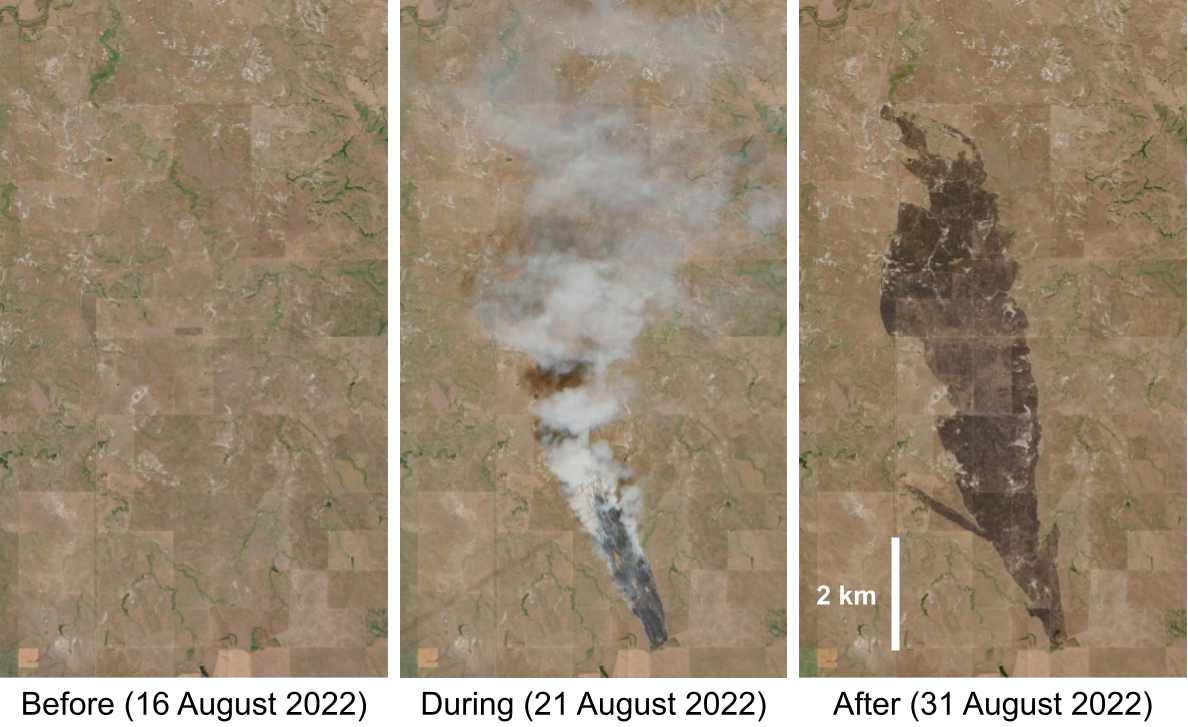
\includegraphics[width=0.99\columnwidth]{SatelliteFireSpread.png}
	\caption{True-color images of a fire in North Dakota, which a satellite from the Sentinel-2 mission caught shortly after the fire started---a tall smoke plume coming off the wind-driven head fire is clearly visible on 21 August 2022.
	NBR and $\Delta$NBR in Figure~\ref{Fig:NBRexample}.  }
	\label{Fig:TrueColor} % Fig.~\ref{Fig:TrueColor}
\end{figure}
\vspace{-12pt}

\begin{figure}[H]
%	\centering
	
\includegraphics[width=0.99\columnwidth]{region_map-1.png}
	\caption{Portions %MDPI: Please confirm if the circle and black-line area need any explanation. Author: OK
 of Montana, North Dakota, and South Dakota encompassed by the primary EPA Level III ecoregions of the Northern Great Plains---Northwestern Glaciated Plains and Northwestern Great Plains---within the broader US Great Plains (inset, red area). 
	Ecoregions shaded by mean total annual precipitation for the complete years in the study period (2017\textendash 2024). 
	$R_{x}$ badges indicate locations of prescribed burn experiments. 
	Open circles denote centroids of wildfire events in the NIFC Interagency Wildfire Perimeter database, 2017--2023; total counts presented in Table~\ref{AppTab:StatesFires}. }
	\label{AppFig:RegionMap} % Fig.~\ref{AppFig:RegionMap}
\end{figure}

\begin{table}[H] 
\caption{Summarized %MDPI: Please confirm the alignment change. Same to the following tables. Author; OK
 totals of wildfire incidents presented in Figure~\ref{AppFig:RegionMap}.  }
\label{AppTab:StatesFires}
\setlength{\cellWidtha}{\textwidth/4-2\tabcolsep-0in}%第一列
\setlength{\cellWidthb}{\textwidth/4-2\tabcolsep--0.2in}%第二列
\setlength{\cellWidthc}{\textwidth/4-2\tabcolsep-0in}%第三列
\setlength{\cellWidthd}{\textwidth/4-2\tabcolsep-0.2in}%第四列
\scalebox{1}[1]{\begin{tabularx}{\textwidth}
{
>{\centering\arraybackslash}m{\cellWidtha}%第一列
>{\centering\arraybackslash}m{\cellWidthb}%第二列
>{\centering\arraybackslash}m{\cellWidthc}%第三列
>{\centering\arraybackslash}m{\cellWidthd}%第四列
}
\toprule
\textbf{State} & \textbf{NW Glaciated Plains} & \textbf{NW Great Plains} & \textbf{Total} \\ 
\midrule
 Montana (MT) & 153 & 998 & 1151 \\ 
South Dakota (SD) &   9 & 339 & 348 \\ 
North Dakota (ND) &  21 & 150 & 171 \\
%\hline
\bottomrule
\end{tabularx}}
\end{table}\vspace{-12pt}

\begin{table}[H] 
	\caption{Monthly %MDPI: Please confirm if abbreviation for month should be completed and unify in the table. Author; OK
 distribution of the wildfire subset used in this study, by zone, as determined by midpoint of pre- and post-fire image dates.  }
	\label{AppTab:FireMonths}
\setlength{\cellWidtha}{\textwidth/10-2\tabcolsep-0in}%第一列
\setlength{\cellWidthb}{\textwidth/10-2\tabcolsep-0in}%第二列
\setlength{\cellWidthc}{\textwidth/10-2\tabcolsep-0in}%第三列
\setlength{\cellWidthd}{\textwidth/10-2\tabcolsep-0in}%第四列
\setlength{\cellWidthe}{\textwidth/10-2\tabcolsep-0in}%第五列
\setlength{\cellWidthf}{\textwidth/10-2\tabcolsep-0in}%第六列
\setlength{\cellWidthg}{\textwidth/10-2\tabcolsep-0in}%第七列
\setlength{\cellWidthh}{\textwidth/10-2\tabcolsep-0in}
\setlength{\cellWidthi}{\textwidth/10-2\tabcolsep-0in}
\setlength{\cellWidthj}{\textwidth/10-2\tabcolsep-0in}
\scalebox{1}[1]{\begin{tabularx}{\textwidth}
{
>{\centering\arraybackslash}m{\cellWidtha}%第一列
>{\centering\arraybackslash}m{\cellWidthb}%第二列
>{\centering\arraybackslash}m{\cellWidthc}%第三列
>{\centering\arraybackslash}m{\cellWidthd}%第四列
>{\centering\arraybackslash}m{\cellWidthe}%第五列
>{\centering\arraybackslash}m{\cellWidthf}%第六列
>{\centering\arraybackslash}m{\cellWidthg}%第七列
>{\centering\arraybackslash}m{\cellWidthh}
>{\centering\arraybackslash}m{\cellWidthi}
>{\centering\arraybackslash}m{\cellWidthj}
}
	\toprule
	\textbf{Zone} & \textbf{Jan} & \textbf{Feb} & \textbf{Mar} & \textbf{Apr} & \textbf{May} & \textbf{Jun} & \textbf{Jul} & \textbf{Aug} & \textbf{Sep} \\ 
	\midrule
	East &   1 &  1 &   1  &   2 &  2 & 0   & 2 &  1 & 0  \\ 
	West &   1 &  0 &   2 &   3 &  0  & 0   & 5 &  6 &  2 \\ 
	\bottomrule
	\end{tabularx}}
\end{table}\vspace{-12pt}

\begin{table}[H] 
	\caption{Summary statistics for three fire behavior measurements made \emph{in agris} and $\Delta$NBR by zone.
	\emph{In agris} fire behavior data from \cite{mcgranahan2023}.  }
	\label{AppTab:FBSum}
\setlength{\cellWidtha}{\textwidth/5-2\tabcolsep-0.4in}%第一列
\setlength{\cellWidthb}{\textwidth/5-2\tabcolsep--0.9in}%第二列
\setlength{\cellWidthc}{\textwidth/5-2\tabcolsep-0.2in}%第三列
\setlength{\cellWidthd}{\textwidth/5-2\tabcolsep-0.1in}%第四列
\setlength{\cellWidthe}{\textwidth/5-2\tabcolsep-0.2in}%第五列
\scalebox{1}[1]{\begin{tabularx}{\textwidth}
{
>{\centering\arraybackslash}m{\cellWidtha}%第一列
>{\raggedright\arraybackslash}m{\cellWidthb}%第二列
>{\centering\arraybackslash}m{\cellWidthc}%第三列
>{\centering\arraybackslash}m{\cellWidthd}%第四列
>{\centering\arraybackslash}m{\cellWidthe}%第五列
}
	\toprule
	\textbf{Zone} & \textbf{Response} & \textbf{Minimum} & \textbf{Mean \boldmath{$\pm$} S.E.} & \textbf{Maximum} \\ 
	\midrule
	East & Flame temperature (\degC) & 55 & 238 $\pm$ 19 & 432 \\ 
	 & Soil surface temperature (\degC) & 17 & 122 $\pm$ 19 & 444 \\  
	 & Rate of spread (m$\cdot$min\textsuperscript{$-$1}) & 0.01 & 3.2 $\pm$ 0.6 & 14.4 \\ 
	& Burn severity ($\Delta$NBR) & 0.06 & 0.24 $\pm$ 0.02 & 0.52 \\
	\midrule
	West & Flame temperature (\degC) & 89 & 282 $\pm$ 16 & 466 \\ 
	 & Soil surface temperature (\degC) & 18 & 177 $\pm$ 25 & 440 \\ 
	 & Rate of spread (m$\cdot$min\textsuperscript{$-$1}) & 0.32 & 4.9 $\pm$ 1.1 & 22.2 \\ 
	 & Burn severity ($\Delta$NBR) & 0.06 & 0.37 $\pm$ 0.02 & 0.51 \\ 
	\bottomrule
\end{tabularx}}
\end{table}\vspace{-12pt}


\begin{table}[H] 
	\caption{Summary statistics for $\Delta$NBR by zone and fire type.  }
	\label{AppTab:WfRxSum}
\setlength{\cellWidtha}{\textwidth/5-2\tabcolsep-0.2in}%第一列
\setlength{\cellWidthb}{\textwidth/5-2\tabcolsep--0.2in}%第二列
\setlength{\cellWidthc}{\textwidth/5-2\tabcolsep-0in}%第三列
\setlength{\cellWidthd}{\textwidth/5-2\tabcolsep-0in}%第四列
\setlength{\cellWidthe}{\textwidth/5-2\tabcolsep-0in}%第五列
\scalebox{1}[1]{\begin{tabularx}{\textwidth}
{
>{\centering\arraybackslash}m{\cellWidtha}%第一列
>{\raggedright\arraybackslash}m{\cellWidthb}%第二列
>{\centering\arraybackslash}m{\cellWidthc}%第三列
>{\centering\arraybackslash}m{\cellWidthd}%第四列
>{\centering\arraybackslash}m{\cellWidthe}%第五列
}
	\toprule
	\textbf{Zone} & \textbf{Fire Type} & \textbf{Minimum} & \textbf{Mean \boldmath{$\pm$} S.E.} & \textbf{Maximum} \\ 
	\midrule
	East & Prescribed burn & 0.1 & 0.2 $\pm$ 0.02 & 0.4 \\ 
	 & Wildfire & 0.4 & 0.5 $\pm$ 0.03 & 0.54 \\ 
	\midrule
	West & Prescribed burn & 0.2 & 0.4 $\pm$ 0.02 & 0.5 \\ 
	 & Wildfire & 0.13 & 0.3 $\pm$ 0.02 & 0.46 \\ 
	\bottomrule
\end{tabularx}}
\end{table}

%%%%%%%%%%%%%%%%%%%%%%%%%%%%%%%


\begin{adjustwidth}{-\extralength}{0cm}

\reftitle{References %MDPI: Please carefully check the refs both in this part and in the main text. Please make sure all refs been cited correctly in sequential numerical order. Our production editor has done thoroughly layout work for the reference. Thanks for your cooperation. Author: OK
}

\begin{thebibliography}{999}

\bibitem[McGranahan and Wonkka(2021)]{mcgranahan2021a}
McGranahan, D.A.; Wonkka, C.L.
\newblock {\em Ecology of {{Fire-Dependent Ecosystems}}: {{Wildland Fire
  Science}}, {{Policy}}, and {{Management}}}; CRC Press: Boca Raton, FL, USA, 2021.

\bibitem[Finney et~al.(2021)Finney, McAllister, Forthofer, and
  Grumstrup]{finney2021}
Finney, M.A.; McAllister, S.S.; Forthofer, J.M.; Grumstrup, T.P.
\newblock {\em Wildland {{Fire Behaviour}}: {{Dynamics}}, {{Principles}} and
  {{Processes}}}; CSIRO Publishing: Melbourne, Australia, %MDPI: Newly added/revised information. Please confirm. Same as below. Author: City corrected as per reference
 2021.

\bibitem[Rothermel and Deeming(1980)]{rothermel1980}
Rothermel, R.C.; Deeming, J.E.
\newblock \emph{Measuring and Interpreting Fire Behavior for Correlation with Fire
  Effects};
\newblock General {{Technical Report}} INT-93; US Department of Agriculture,
  Forest Service, Intermountain Forest and Range Experiment Station: Ogden, UT, USA,~1980.

\bibitem[{ILRI, IUCN, FAO, WWF, UNEP and ILC}(2021)]{ilri2021}
{ILRI; IUCN; FAO; WWF; UNEP; ILC}.
\newblock \emph{Rangeland Atlas};
\newblock Technical Report; International Livestock Research Institute:
  Nairobi, Kenya,  2021.

\bibitem[Vaartaja(1949)]{vaartaja1949}
Vaartaja, O.
\newblock High {{Surface Soil Temperatures}} on {{Methods}} of
  {{Investigation}}, and {{Thermocouple Observations}} on a {{Wooded Heath}} in
  the {{South}} of {{Finland}}.
\newblock {\em Oikos} {\bf 1949}, {\em 1},~6.
\url{https://doi.org/10.2307/3565034}.

\bibitem[Engle et~al.(1989)Engle, Bidwell, Ewing, and Williams]{engle1989}
Engle, {\relax D.M}.; Bidwell, {\relax T.G}.; Ewing, {\relax A.L}.; Williams,
  {\relax JR}.
\newblock A Technique for Quantifying Fire Behavior in Grassland Fire Ecology
  Studies.
\newblock {\em  Southwest. Nat.} {\bf 1989}, {\em 34},~79--84.

\bibitem[McGranahan(2020)]{mcgranahan2020a}
McGranahan, D.A.
\newblock An Inconvenient Truth about Temperature-Time Data from Thermocouples.
\newblock {\em Plant Ecol.} {\bf 2020}, {\em 221},~1091--1104.
\newblock
\url{https://doi.org/10.1007/s11258-020-01064-7}.

\bibitem[Pavlasek et~al.(2015)Pavlasek, Elliott, Pearce, Duris, Palencar,
  Koval, and Machin]{pavlasek2015}
Pavlasek, P.; Elliott, C.J.; Pearce, J.V.; Duris, S.; Palencar, R.; Koval, M.;
  Machin, G.
\newblock Hysteresis {{Effects}} and {{Strain-Induced Homogeneity Effects}} in
  {{Base Metal Thermocouples}}.
\newblock {\em Int. J. Thermophys.} {\bf 2015}, {\em
  36},~467--481.
\newblock
  \url{https://doi.org/10.1007/s10765-015-1841-3}.

\bibitem[Shannon and Butler(2003-11-16/2003-11-20)]{shannon2003}
Shannon, K.S.; Butler, B.W.
\newblock A Review of Error Associated with Thermocouple Temperature
  Measurement in Fire Environments.
\newblock  In \emph{Proceedings of the 2nd Fire Ecology Congress}; American
  Meteorological Society: Orlando, FL, USA, 2003; p. 3.


\bibitem[Walker and Stocks(1968)]{walker1968}
Walker, {\relax J.D}.; Stocks, {\relax B.J}.
\newblock Thermocouple Errors in Forest Fire Research.
\newblock {\em Fire Technol.} {\bf 1968}, {\em 4},~59--62.

\bibitem[Lemaire and Menanteau(2017)]{lemaire2017}
Lemaire, R.; Menanteau, S.
\newblock Assessment of Radiation Correction Methods for Bare Bead
  Thermocouples in a Combustion Environment.
\newblock {\em Int. J. Therm. Sci.} {\bf 2017}, {\em
  122},~186--200.
\newblock
  \url{https://doi.org/10.1016/j.ijthermalsci.2017.08.014}.

\bibitem[Blevins and Pitts(1999)]{blevins1999}
Blevins, L.G.; Pitts, W.M.
\newblock Modeling of Bare and Aspirated Thermocouples in Compartment Fires.
\newblock {\em Fire Saf. J.} {\bf 1999}, {\em 33},~239--259.

\bibitem[Smith et~al.(2016)Smith, Cowan, and Fitzgerald]{smith2016}
Smith, J.E.; Cowan, A.D.; Fitzgerald, S.A.
\newblock Soil Heating during the Complete Combustion of Mega-Logs and
  Broadcast Burning in Central {{Oregon USA}} Pumice Soils.
\newblock {\em Int. J. Wildland Fire} {\bf 2016}, {\em
  25},~1202.
\newblock
  \url{https://doi.org/10.1071/WF16016}.

\bibitem[Pingree and Kobziar(2019)]{pingree2019}
Pingree, M.R.; Kobziar, L.N.
\newblock The Myth of the Biological Threshold: {{A}} Review of Biological
  Responses to Soil Heating Associated with Wildland Fire.
\newblock {\em For. Ecol. Manag.} {\bf 2019}, {\em
  432},~1022--1029.
\newblock
  \url{https://doi.org/10.1016/j.foreco.2018.10.032}.

\bibitem[Wright(1970)]{wright1970}
Wright, H.A.
\newblock A {{Method}} to {{Determine Heat-Caused Mortality}} in
  {{Bunchgrasses}}.
\newblock {\em Ecology} {\bf 1970}, {\em 51},~582--587.
\newblock
  \url{https://doi.org/10.2307/1934038}.

\bibitem[Dickinson and Johnson(2004)]{dickinson2004}
Dickinson, M.B.; Johnson, E.A.
\newblock Temperature-Dependent Rate Models of Vascular Cambium Cell Mortality.
\newblock {\em Can. J. For. Res.} {\bf 2004}, {\em
  34},~546--559.
\newblock
  \url{https://doi.org/10.1139/x03-223}.

\bibitem[Bova and Dickinson(2005)]{bova2005}
Bova, A.S.; Dickinson, M.B.
\newblock Linking Surface-Fire Behavior, Stem Heating, and Tissue Necrosis.
\newblock {\em Can. J. For. Res.} {\bf 2005}, {\em
  35},~814--822.
\newblock
  \url{https://doi.org/10.1139/x05-004}.

\bibitem[Alexander(1982)]{alexander1982}
Alexander, M.E.
\newblock Calculating and Interpreting Forest Fire Intensities.
\newblock {\em Can. J. Bot.} {\bf 1982}, {\em 60},~349--357.

\bibitem[Bova and Dickinson(2008)]{bova2008}
Bova, A.S.; Dickinson, M.B.
\newblock Beyond ``Fire Temperatures'': Calibrating Thermocouple Probes and
  Modeling Their Response to Surface Fires in Hardwood Fuels.
\newblock {\em Can. J. For. Res.} {\bf 2008}, {\em
  38},~1008--1020.
\newblock
  \url{https://doi.org/10.1139/X07-204}.

\bibitem[Byram(1959)]{byram1959}
Byram, G.
\newblock Combustion of Forest Fuels.
\newblock In {\em Forest Fire: Control and Use}; McGraw-Hill Book Company Inc.: London, UK,
 {1959}; pp.~61--89.

\bibitem[Perry(1998)]{perry1998}
Perry, G.L.W.
\newblock Current Approaches to Modelling the Spread of Wildland Fire: A
  Review.
\newblock {\em Prog. Phys. Geogr.} {\bf 1998}, {\em 22},~222--245.

\bibitem[Cruz et~al.(2018)Cruz, Alexander, Sullivan, Gould, and
  Kilinc]{cruz2018}
Cruz, M.G.; Alexander, M.E.; Sullivan, A.L.; Gould, J.S.; Kilinc, M.
\newblock Assessing Improvements in Models Used to Operationally Predict
  Wildland Fire Rate of Spread.
\newblock {\em Environ. Model. Softw.} {\bf 2018}, {\em
  105},~54--63.
\newblock
  \url{https://doi.org/10.1016/j.envsoft.2018.03.027}.

\bibitem[Simard et~al.(1982)Simard, Deacon, and Adams]{simard1982}
Simard, A.J.; Deacon, A.G.; Adams, K.B.
\newblock Nondirectional Sampling of Wildland Fire Spread.
\newblock {\em Fire Technol.} {\bf 1982}, {\em 18},~221--228.
\newblock
  \url{https://doi.org/10.1007/BF02473134}.

\bibitem[Simard et~al.(1984)Simard, Eenigenburg, Adams, Nissen~Jr, and
  Deacon]{simard1984}
Simard, A.J.; Eenigenburg, J.E.; Adams, K.B.; Nissen, R.L., Jr.; Deacon, A.G.
\newblock A General Procedure for Sampling and Analyzing Wildland Fire Spread.
\newblock {\em For. Sci.} {\bf 1984}, {\em 30},~51--64.

\bibitem[Clements et~al.(2019)Clements, Kochanski, Seto, Davis, Camacho,
  Lareau, Contezac, Restaino, Heilman, Krueger, Butler, Ottmar, Vihnanek,
  Flynn, Filippi, Barboni, Hall, Mandel, Jenkins, O'Brien, Hornsby, and
  Teske]{clements2019}
Clements, C.B.; Kochanski, A.K.; Seto, D.; Davis, B.; Camacho, C.; Lareau,
  N.P.; Contezac, J.; Restaino, J.; Heilman, W.E.; Krueger, S.K.; et al.
\newblock The {{FireFlux II}} Experiment: A Model-Guided Field Experiment to
  Improve Understanding of Fire--Atmosphere Interactions and Fire Spread.
\newblock {\em Int. J. Wildland Fire} {\bf 2019}, {\em
  28},~308--326.
\newblock
  \url{https://doi.org/10.1071/WF18089}.

\bibitem[McGranahan(2021)]{mcgranahan2021}
McGranahan, D.A.
\newblock {{FeatherFlame}}: {{An Arduino-based}} Thermocouple Datalogging
  System to Record Wildland Fire Flame Temperatures {{{\emph{in agris}}}.}
\newblock {\em Rangel. Ecol. Manag.} {\bf 2021}, {\em 76},~43--47.

\bibitem[McGranahan et~al.(2023)McGranahan, Zopfi, and
  Yurkonis]{mcgranahan2023}
McGranahan, D.A.; Zopfi, M.E.; Yurkonis, K.A.
\newblock Weather and Fuel as Modulators of Grassland Fire Behavior in the
  Northern {{Great Plains}}.
\newblock {\em Environ. Manag.} {\bf 2023}, {\em 71},~940--949.
\newblock
  \url{https://doi.org/10.1007/s00267-022-01767-9}.

\bibitem[Finney and Martin(1992)]{finney1992}
Finney, M.A.; Martin, R.E.
\newblock Calibration and Field Testing of Passive Flame Height Sensors.
\newblock {\em Int. J. Wildland Fire} {\bf 1992}, {\em
  2},~115--122.

\bibitem[Szpakowski and Jensen(2019)]{szpakowski2019}
Szpakowski, D.M.; Jensen, J.L.R.
\newblock A {{Review}} of the {{Applications}} of {{Remote Sensing}} in {{Fire
  Ecology}}.
\newblock {\em Remote Sens.} {\bf 2019}, {\em 11},~2638.
\newblock
  \url{https://doi.org/10.3390/rs11222638}.

\bibitem[Key and Benson(2006)]{key2006a}
Key, C.H.; Benson, N.C.
\newblock Landscape Assessment: Remote Sensing of Severity, the Normalized Burn
  Ratio and Ground Measure of Severity, the Composite Burn Index. In {\em
  {{FIREMON}}: {{Fire}} Effects Monitoring and Inventory System}; General Technical Report RMRS-GTR-164-CD; Lutes, D.C., Keane, R.E., Caratti,
  J.F., Key, C.H., Benson, N.C., Sutherland, S., Gangi, L.J., Eds.; USDA Forest
  Service, Rocky Mountain Research Station: Fort Collins, CO, USA, 2006; pp.~ LA--1--55. %MDPI: Please check if the page range is correct. Author: Correct


\bibitem[Veraverbeke et~al.(2010)Veraverbeke, Lhermitte, Verstraeten, and
  Goossens]{veraverbeke2010}
Veraverbeke, S.; Lhermitte, S.; Verstraeten, W.W.; Goossens, R.
\newblock The Temporal Dimension of Differenced {{Normalized Burn Ratio}}
  ({{dNBR}}) Fire/Burn Severity Studies: {{The}} Case of the Large 2007
  {{Peloponnese}} Wildfires in {{Greece}}.
\newblock {\em Remote Sens. Environ.} {\bf 2010}, {\em
  114},~2548--2563.
\newblock
  \url{https://doi.org/10.1016/j.rse.2010.05.029}.

\bibitem[Eidenshink et~al.(2007)Eidenshink, Schwind, Brewer, Zhu, Quayle,
  and Howard]{eidenshink2007a}
Eidenshink, J.; Schwind, B.; Brewer, K.; Zhu, Z.L.; Quayle, B.; Howard, S.
\newblock A Project for Monitoring Trends in Burn Severity.
\newblock {\em Fire Ecol.} {\bf 2007}, {\em 3},~3--21.

\bibitem[Lentile et~al.(2006)Lentile, Holden, Smith, Falkowski, Hudak,
  Morgan, Lewis, Gessler, and Benson]{lentile2006}
Lentile, L.B.; Holden, Z.A.; Smith, A.M.S.; Falkowski, M.J.; Hudak, A.T.;
  Morgan, P.; Lewis, S.A.; Gessler, P.E.; Benson, N.C.
\newblock Remote Sensing Techniques to Assess Active Fire Characteristics and
  Post-Fire Effects.
\newblock {\em Int. J. Wildland Fire} {\bf 2006}, {\em
  15},~319--345.
\newblock
  \url{https://doi.org/10.1071/WF05097}.

\bibitem[Donovan and Brown(2007)]{donovan2007}
Donovan, G.H.; Brown, T.C.
\newblock Be Careful What You Wish for: The Legacy of {{Smokey Bear}}.
\newblock {\em Front. Ecol. Environ.} {\bf 2007}, {\em
  5},~73--79.
\newblock
  \url{https://doi.org/10.1890/1540-9295(2007)5[73:BCWYWF]2.0.CO;2}.

\bibitem[Parks et~al.(2015)Parks, Miller, Parisien, Holsinger, Dobrowski,
  and Abatzoglou]{parks2015}
Parks, S.A.; Miller, C.; Parisien, M.A.; Holsinger, L.M.; Dobrowski, S.Z.;
  Abatzoglou, J.
\newblock Wildland Fire Deficit and Surplus in the Western {{United States}},
  1984--2012.
\newblock {\em Ecosphere} {\bf 2015}, {\em 6},~1--13.
\newblock
  \url{https://doi.org/10.1890/ES15-00294.1}.

\bibitem[Kolden(2019)]{kolden2019}
Kolden, C.A.
\newblock We're {{Not Doing Enough Prescribed Fire}} in the {{Western United
  States}} to {{Mitigate Wildfire Risk}}.
\newblock {\em Fire} {\bf 2019}, {\em 2},~30.
\newblock
  \url{https://doi.org/10.3390/fire2020030}.

\bibitem[Fernandes and Botelho(2003)]{fernandes2003}
Fernandes, P.M.; Botelho, H.S.
\newblock A Review of Prescribed Burning Effectiveness in Fire Hazard
  Reduction.
\newblock {\em Int. J. Wildland Fire} {\bf 2003}, {\em
  12},~117--128.
\newblock
  \url{https://doi.org/10.1071/wf02042}.

\bibitem[Brodie et~al.(2024)Brodie, Knapp, Brooks, Drury, and
  Ritchie]{brodie2024}
Brodie, E.G.; Knapp, E.E.; Brooks, W.R.; Drury, S.A.; Ritchie, M.W.
\newblock Forest Thinning and Prescribed Burning Treatments Reduce Wildfire
  Severity and Buffer the Impacts of Severe Fire Weather.
\newblock {\em Fire Ecol.} {\bf 2024}, {\em 20},~17.
\newblock
  \url{https://doi.org/10.1186/s42408-023-00241-z}.

\bibitem[McGranahan and Angerer(2025)]{mcgranahan2025}
McGranahan, D.A.; Angerer, J.P.
\newblock Evaluating an Attempt to Restore Summer Fire in the {{Northern Great
  Plains}}.
\newblock {\em Environ. Manag.} {\bf 2025}, {\em 75},~1656--1664.
\newblock
  \url{https://doi.org/10.1007/s00267-025-02209-y}.

\bibitem[{R Core Team}(2024)]{rcoreteam2024}
{R Core Team}.
\newblock {\em R: A Language and Environment for Statistical Computing} v.4.6.0;
\newblock R Foundation for Statistical Computing:
 Vienna, Austria,  2024.

\bibitem[McGranahan(2025)]{mcgranahan2025b}
McGranahan, D.A.
\newblock Data from: Remote Sensing in Rangeland Fire Ecology:
  Comparing Imagery to Measured Fire Behavior, and Burn Severity Across
  Prescribed Burns and Wildfires,  2026.
\newblock Ag Data Commons. Dataset. 
\newblock \url{https://doi.org/10.15482/USDA.ADC/30037582}
%MDPI: !!Please provide more information about the article type, such as 
%book (please provide the name and location of the publisher); 
%online resource (please provide the URL of the website and the date it was accessed (Date Month Year)); 
%or journal article (please provide the name of the journal, the year and volume in which it was published, and the page number). Please refer to https://www.mdpi.com/authors/references for full reference formatting guides.
% Author: Your citation reference does not include a citation format for data repositories. Edit added information as necessary.

\bibitem[Duquette et~al.(2022)Duquette, McGranahan, Wanchuk, Hovick, Limb,
  and Sedivec]{duquette2022}
Duquette, C.; McGranahan, D.A.; Wanchuk, M.; Hovick, T.; Limb, R.; Sedivec, K.
\newblock Heterogeneity-Based Management Restores Diversity and Alters
  Vegetation Structure without Decreasing Invasive Grasses in Working
  Mixed-Grass Prairie.
\newblock {\em Land} {\bf 2022}, {\em 11},~1135.
\newblock
  \url{https://doi.org/10.3390/land11081135}.

\bibitem[Wanchuk et~al.(2024)Wanchuk, McGranahan, Sedivec, Berti, Swanson,
  and Hovick]{wanchuk2024}
Wanchuk, M.R.; McGranahan, D.A.; Sedivec, K.K.; Berti, M.; Swanson, K.C.;
  Hovick, T.J.
\newblock Improving Forage Nutritive Value and Livestock Performance with
  Spatially-Patchy Prescribed Fire in Grazed Rangeland.
\newblock {\em Agric. Ecosyst. Environ.} {\bf 2024}, {\em
  368},~109004.
\newblock
  \url{https://doi.org/10.1016/j.agee.2024.109004}.

\bibitem[McGranahan(2025)]{mcgranahan2025a}
McGranahan, D.A.
\newblock Spatially-Discrete Disturbance Overrides Inherent Environmental
  Heterogeneity in Grazed Mixed-Grass Prairie.
\newblock {\em Oikos} {\bf 2025}, {\em 2025},~e11195.
\newblock
  \url{https://doi.org/10.1111/oik.11195}.

\bibitem[Spiess et~al.(2024)Spiess, McGranahan, Geaumont, Berti, Gasch,
  and Hovick]{spiess2024}
Spiess, J.W.; McGranahan, D.A.; Geaumont, B.; Berti, M.; Gasch, C.; Hovick,
  T.J.
\newblock Spatio-Temporal Patterns of Rangeland Forage Nutritive Value and
  Grazer Selection with Patch-Burning in the {{US}} Northern {{Great Plains}}.
\newblock {\em J. Environ. Manag.} {\bf 2024}, {\em
  357},~120731.
\newblock
  \url{https://doi.org/10.1016/j.jenvman.2024.120731}.

\bibitem[Spiess et~al.(2025)Spiess, McGranahan, Hovick, Berti, Gasch, and
  Geaumont]{spiess2025}
Spiess, J.W.; McGranahan, D.A.; Hovick, T.; Berti, M.; Gasch, C.; Geaumont, B.
\newblock Patch-{{Burn Grazing Increased Structural Heterogeneity}} in
  {{Southwestern North Dakota Rangelands}}.
\newblock {\em Appl. Veg. Sci.} {\bf 2025}, {\em 28},~e70016.
\newblock
  \url{https://doi.org/10.1111/avsc.70016}.

\bibitem[McGranahan et~al.(2022)McGranahan, Wonkka, Dangi, Spiess, and
  Geaumont]{mcgranahan2022}
McGranahan, D.A.; Wonkka, C.L.; Dangi, S.; Spiess, J.W.; Geaumont, B.
\newblock Mineral Nitrogen and Microbial Responses to Soil Heating in Burned
  Grassland.
\newblock {\em Geoderma} {\bf 2022}, {\em 424},~116023.
\newblock
  \url{https://doi.org/10.1016/j.geoderma.2022.116023}.

\bibitem[{National Interagency Fire Center}(2024)]{nifc2024}
{National Interagency Fire Center}.
\newblock {{InterAgencyFirePerimeterHistory All Years}}.  2024.
\newblock
  Avaailable online: \url{https://data-nifc.opendata.arcgis.com/datasets/nifc::interagencyfireperimeterhistory-all-years-view/explore?location=29.282787,-122.087025,3.64} (accessed on 5 August 2025).
%MDPI: -Please add the access date, e.g., “URL (accessed on 1 January 2020)” (should be before 8 May 2026). Same as below.
%-Please ensure that all webs in the text are accessible.
 

\bibitem[{USDA Forest Service}(no date)]{usdaforestservicenodate}
{USDA Forest Service}.
\newblock Rangelands.
\newblock Avaailable online: \url{https://data.fs.usda.gov/geodata/rastergateway/rangelands/index.php} (accessed on 2 November 2023).


\bibitem[{NDAWN}(2025{\natexlab{a}})]{ndawn2025}
{NDAWN}.
\newblock NDAWN Daily Data for Streeter, ND, 1 January 2017 to
  31 December 2024.  2025. 
\newblock North Dakota Agricultural Weather Network. Dataset. 
\newblock Available online: \url{https://ndawn.ndsu.nodak.edu/get-table.html?station=48&variable=ddavt&variable=ddr&year=2025&ttype=daily&quick_pick=&begin_date=2017-01-01&end_date=2024-12-31} (accessed on 5 August 2025).
%MDPI: !!Please provide more information about the article type, such as 
%book (please provide the name and location of the publisher); 
%online resource (please provide the URL of the website and the date it was accessed (Date Month Year)); 
%or journal article (please provide the name of the journal, the year and volume in which it was published, and the page number). Please refer to https://www.mdpi.com/authors/references for full reference formatting guides.


\bibitem[{NDAWN}(2025{\natexlab{b}})]{ndawn2025a}
{NDAWN}.
\newblock NDAWN Daily Data for Hettinger, ND, 1 January 2017
  to 31 December 2024.  2025.
\newblock North Dakota Agricultural Weather Network. Dataset. 
\newblock Available online: \url{https://ndawn.ndsu.nodak.edu/get-table.html?station=29&variable=ddavt&variable=ddr&year=2025&ttype=daily&quick_pick=&begin_date=2017-01-01&end_date=2024-12-31} (accessed on 5 August 2025).
%MDPI: !!Please provide more information about the article type, such as 
%book (please provide the name and location of the publisher); 
%online resource (please provide the URL of the website and the date it was accessed (Date Month Year)); 
%or journal article (please provide the name of the journal, the year and volume in which it was published, and the page number). Please refer to https://www.mdpi.com/authors/references for full reference formatting guides.

\bibitem[Abatzoglou et~al.(2018)Abatzoglou, Dobrowski, Parks, and
  Hegewisch]{abatzoglou2018}
Abatzoglou, J.T.; Dobrowski, S.Z.; Parks, S.A.; Hegewisch, K.C.
\newblock {{TerraClimate}}, a High-Resolution Global Dataset of Monthly Climate
  and Climatic Water Balance from 1958--2015.
\newblock {\em Sci. Data} {\bf 2018}, {\em 5},~170191.
\newblock
  \url{https://doi.org/10.1038/sdata.2017.191}.

\bibitem[Johnson(2021)]{johnson2021}
Johnson, M.
\newblock climateR: An R Package for Getting Point and Gridded Climate
  Data by AOI.  2021.
\newblock R package version 0.3.6. 
\newblock Available online: \url{https://github.com/mikejohnson51/climateR} (accessed on 5 August 2025).
%MDPI: !!Please provide more information about the article type, such as 
%book (please provide the name and location of the publisher); 
%online resource (please provide the URL of the website and the date it was accessed (Date Month Year)); 
%or journal article (please provide the name of the journal, the year and volume in which it was published, and the page number). Please refer to https://www.mdpi.com/authors/references for full reference formatting guides.


\bibitem[{United States Geological Survey}(no date)]{usgs_nm}
{United States Geological Survey}.
\newblock {{USGSImageryOnly}} ({{MapServer}}).
\newblock
  Available online: \url{https://basemap.nationalmap.gov/arcgis/rest/services/USGSImageryOnly/MapServer} (accessed on 5 August 2025).

\bibitem[Llorens et~al.(2021)Llorens, Sobrino, Fern{\'a}ndez,
  {Fern{\'a}ndez-Alonso}, and Vega]{llorens2021}
Llorens, R.; Sobrino, J.A.; Fern{\'a}ndez, C.; {Fern{\'a}ndez-Alonso}, J.M.;
  Vega, J.A.
\newblock A Methodology to Estimate Forest Fires Burned Areas and Burn Severity
  Degrees Using {{Sentinel-2}} Data. {{Application}} to the {{October}} 2017
  Fires in the {{Iberian Peninsula}}.
\newblock {\em Int. J. Appl. Earth Obs. Geoinf.} {\bf 2021}, {\em 95},~102243.
\newblock
  \url{https://doi.org/10.1016/j.jag.2020.102243}.

\bibitem[Schott et~al.(1988)Schott, Salvaggio, and Volchok]{schott1988}
Schott, J.R.; Salvaggio, C.; Volchok, W.J.
\newblock Radiometric Scene Normalization Using Pseudoinvariant Features.
\newblock {\em Remote Sens. Environ.} {\bf 1988}, {\em 26},~1--16.
\newblock
  \url{https://doi.org/10.1016/0034-4257(88)90116-2}.

\bibitem[Hijmans et~al.(2022)Hijmans, Bivand, Forner, Ooms, Pebesma, and
  Sumner]{hijmans2022}
Hijmans, R.J.; Bivand, R.; Forner, K.; Ooms, J.; Pebesma, E.; Sumner, M.D.
\newblock terra: Spatial Data Analysis.  2025.
\newblock R package version 1.8-60. 
\newblock Available online: \url{https://CRAN.R-project.org/package=terra} (accessed on 5 August 2025).
%MDPI: !!Please provide more information about the article type, such as 
%book (please provide the name and location of the publisher); 
%online resource (please provide the URL of the website and the date it was accessed (Date Month Year)); 
%or journal article (please provide the name of the journal, the year and volume in which it was published, and the page number). Please refer to https://www.mdpi.com/authors/references for full reference formatting guides.


\bibitem[Bates et~al.(2015)Bates, M{\"a}chler, Bolker, and
  Walker]{bates2015}
Bates, D.; M{\"a}chler, M.; Bolker, B.; Walker, S.
\newblock Fitting Linear Mixed-Effects Models Using Lme4.
\newblock {\em J. Stat. Softw.} {\bf 2015}, {\em 67},~1--48.
\newblock
  \url{https://doi.org/10.18637/jss.v067.i01}.

\bibitem[Fox and Weisberg(2019)]{fox2019a}
Fox, J.; Weisberg, S.
\newblock {\em An {{R}} Companion to Applied Regression}, 3rd ed.; Sage: Thousand
  Oaks, CA,  USA, 2019.

\bibitem[Barto{\'n}(2026)]{barton2026}
Barto{\'n}, K.
\newblock  {{MuMIn}}: {{Multi-Model}} Inference.  2026. 
\newblock R package version 1.48.19. 
\newblock Available online: \url{https://CRAN.R-project.org/package=MuMIn} (accessed 23 April 2026).
%MDPI: !!Please provide more information about the article type, such as 
%book (please provide the name and location of the publisher); 
%online resource (please provide the URL of the website and the date it was accessed (Date Month Year)); 
%or journal article (please provide the name of the journal, the year and volume in which it was published, and the page number). Please refer to https://www.mdpi.com/authors/references for full reference formatting guides.


\bibitem[Lenth et~al.(2018)Lenth, Singmann, Love, Buerkner, and
  Herve]{lenth2018}
Lenth, R.; Singmann, H.; Love, J.; Buerkner, P.; Herve, M.
\newblock emmeans: {{Estimated Marginal Means, aka Least-Squares Means}}.
  2024.
 \newblock R package version 1.10.4.
 \newblock Available online: \url{https://CRAN.R-project.org/package=emmeans} (accessed on 11 May 2026).
%MDPI: !!Please provide more information about the article type, such as 
%book (please provide the name and location of the publisher); 
%online resource (please provide the URL of the website and the date it was accessed (Date Month Year)); 
%or journal article (please provide the name of the journal, the year and volume in which it was published, and the page number). Please refer to https://www.mdpi.com/authors/references for full reference formatting guides.


\bibitem[Trollope(1978)]{trollope1978}
Trollope, W.
\newblock Fire Behaviour---{{A}} Preliminary Study.
\newblock {\em Proc. Annu. Congr. Grassl. Soc. South. Afr.} {\bf 1978}, {\em 13},~123--128.
\newblock
  \url{https://doi.org/10.1080/00725560.1978.9648846}.

\bibitem[Trollope(1984)]{trollope1984}
Trollope, W.S.W.
\newblock Fire Behaviour. In {\em Ecological Effects of Fire in {{South
  African}} Ecosystems}; {de V. Booysen}, P., Tainton, N.M., Eds.; Springer: Berlin/Heidelberg, Germany,
  1984; Volume~48, pp. 199--218.

\bibitem[{Gimeno-Garc{\'{\i}}a} et~al.(2004){Gimeno-Garc{\'{\i}}a},
  Andreu, and Rubio]{gimeno-garcia2004}
{Gimeno-Garc{\'{\i}}a}, E.; Andreu, V.; Rubio, J.L.
\newblock Spatial Patterns of Soil Temperatures during Experimental Fires.
\newblock {\em Geoderma} {\bf 2004}, {\em 118},~17--38.
\newblock
  \url{https://doi.org/10.1016/S0016-7061(03)00167-8}.

\bibitem[Schwilk and Caprio(2011)]{schwilk2011}
Schwilk, D.W.; Caprio, A.C.
\newblock Scaling from Leaf Traits to Fire Behaviour: Community Composition
  Predicts Fire Severity in a Temperate Forest.
\newblock {\em J. Ecol.} {\bf 2011}, {\em 99},~970--980.
\newblock
  \url{https://doi.org/10.1111/j.1365-2745.2011.01828.x}.

\bibitem[Yurkonis et~al.(2019)Yurkonis, Dillon, McGranahan, Toledo, and
  Goodwin]{yurkonis2019}
Yurkonis, K.A.; Dillon, J.; McGranahan, D.A.; Toledo, D.; Goodwin, B.J.
\newblock Seasonality of Prescribed Fire Weather Windows and Predicted Fire
  Behavior in the Northern {{Great Plains}}, {{USA}}.
\newblock {\em Fire Ecol.} {\bf 2019}, {\em 15},~7.
\newblock
  \url{https://doi.org/10.1186/s42408-019-0027-y}.

\bibitem[Bosy and Reader(1995)]{bosy1995}
Bosy, J.L.; Reader, R.J.
\newblock Mechanisms {{Underlying}} the {{Suppression}} of {{Forb Seedling
  Emergence}} by {{Grass}} (\textit{{{Poa}} pratensis}) {{Litter}}.
\newblock {\em Funct. Ecol.} {\bf 1995}, {\em 9},~635--639.
  \url{https://doi.org/10.2307/2390155}.

\bibitem[Nouwakpo et~al.(2019)Nouwakpo, Toledo, Sanderson, and
  Weltz]{nouwakpo2019}
Nouwakpo, S.; Toledo, D.; Sanderson, M.; Weltz, M.
\newblock Understanding the Effects of Grazing and Prescribed Fire on Hydrology
  of {{Kentucky}} Bluegrass--Dominated Rangelands in the Northern {{Great
  Plains}}.
\newblock {\em J. Soil Water Conserv.} {\bf 2019}, {\em
  74},~360--371.
\newblock
  \url{https://doi.org/10.2489/jswc.74.4.360}.

\bibitem[Gerhard et~al.(2022)Gerhard, Gasch, and Sedivec]{gerhard2022}
Gerhard, L.; Gasch, C.K.; Sedivec, K.
\newblock Soil Properties Are Resilient despite Grass Invasion, Fire, and
  Grazing.
\newblock {\em Agrosyst. Geosci. Environ.} {\bf 2022}, {\em
  5},~e20257.
\newblock
  \url{https://doi.org/10.1002/agg2.20257}.

\bibitem[Kjaer et~al.(2025)Kjaer, Hovick, Sedivec, and Limb]{kjaer2025}
Kjaer, E.L.; Hovick, T.J.; Sedivec, K.; Limb, R.F.
\newblock Invasive Grass Litter Controls Rangeland Plant Community Dynamics.
\newblock {\em J. Environ. Manag.} {\bf 2025}, {\em
  395},~127755.
\newblock
  \url{https://doi.org/10.1016/j.jenvman.2025.127755}.

\bibitem[Shearman et~al.(1980)Shearman, Kinbacher, Riordan, and
  Steinegger]{shearman1980}
Shearman, R.C.; Kinbacher, E.J.; Riordan, T.P.; Steinegger, D.H.
\newblock Thatch {{Accumulation}} in {{Kentucky Bluegrass}} as {{Influenced}}
  by {{Cultivar}}, {{Mowing}}, and {{Nitrogen1}}.
\newblock {\em HortScience} {\bf 1980}, {\em 15},~312--313.
\newblock
  \url{https://doi.org/10.21273/HORTSCI.15.3.312}.

\bibitem[Docherty et~al.(2012)Docherty, Balser, Bohannan, and
  Gutknecht]{docherty2012}
Docherty, K.M.; Balser, T.C.; Bohannan, B.J.M.; Gutknecht, J.L.M.
\newblock Soil Microbial Responses to Fire and Interacting Global Change
  Factors in a {{California}} Annual Grassland.
\newblock {\em Biogeochemistry} {\bf 2012}, {\em 109},~63--83.
\newblock
  \url{https://doi.org/10.1007/s10533-011-9654-3}.

\bibitem[Egidi et~al.(2016)Egidi, {McMullan-Fisher}, Morgan, May, Zeeman,
  and Franks]{egidi2016}
Egidi, E.; {McMullan-Fisher}, S.; Morgan, J.W.; May, T.; Zeeman, B.; Franks,
  A.E.
\newblock Fire Regime, Not Time-since-Fire, Affects Soil Fungal Community
  Diversity and Composition in Temperate Grasslands.
\newblock {\em FEMS Microbiol. Lett.} {\bf 2016}, {\em 363},~fnw196.
\newblock
  \url{https://doi.org/10.1093/femsle/fnw196}.

\bibitem[Neary et~al.(1999)Neary, Klopatek, DeBano, and
  Ffolliott]{neary1999a}
Neary, D.G.; Klopatek, C.C.; DeBano, L.F.; Ffolliott, P.F.
\newblock Fire Effects on Belowground Sustainability: A Review and Synthesis.
\newblock {\em For. Ecol. Manag.} {\bf 1999}, {\em 122},~51--71.
\newblock
  \url{https://doi.org/10.1016/S0378-1127(99)00032-8}.

\bibitem[Robichaud et~al.(2000)Robichaud, Beyers, and
  Neary]{robichaud2000}
Robichaud, P.R.; Beyers, J.L.; Neary, D.G.
\newblock \emph{Evaluating the Effectiveness of Postfire Rehabilitation Treatments};
\newblock General {{Technical Report}} RMRS-GTR-63; USDA Forest Service, Rocky
  Mountain Research Station: Fort Collins, CO, USA, 2000.

\bibitem[Courtwright(2007)]{courtwright2007}
Courtwright, J.
\newblock ``{{When We First Come Here It All Looked Like Prairie Land
  Almost}}'': {{Prairie Fire}} and {{Plains Settlement}}.
\newblock {\em West. Hist. Q.} {\bf 2007}, {\em 38},~157--179.

\bibitem[Higgins(1984)]{higgins1984}
Higgins, K.F.
\newblock Lightning {{Fires}} in {{North Dakota Grasslands}} and in
  {{Pine-Savanna Lands}} of {{South Dakota}} and {{Montana}}.
\newblock {\em J. Range Manag.} {\bf 1984}, {\em 37},~100--103.
\newblock
  \url{https://doi.org/10.2307/3898892}.

\bibitem[Umbanhowar(1996)]{umbanhowar1996}
Umbanhowar, C.E.
\newblock Recent {{Fire History}} of the {{Northern Great Plains}}.
\newblock {\em Am. Midl. Nat.} {\bf 1996}, {\em 135},~115. 
  \url{https://doi.org/10.2307/2426877}.

\bibitem[Boland et~al.(2025)Boland, McGranahan, Geaumont, Wonkka, Ott, and
  Kreuter]{boland2025}
Boland, K.; McGranahan, D.A.; Geaumont, B.; Wonkka, C.L.; Ott, J.P.; Kreuter,
  U.P.
\newblock Perceptions of Prescribed Fire among Ranchers near Northern {{US
  National Grasslands}}.
\newblock {\em Fire} {\bf 2025}, {\em 8},~102.
\newblock
  \url{https://doi.org/10.3390/fire8030102}.

\bibitem[Spiess et~al.(2020)Spiess, McGranahan, Geaumont, Hovick, Berti,
  Lakey, Sedivec, and Limb]{spiess2020}
Spiess, J.W.; McGranahan, D.A.; Geaumont, B.; Hovick, T.; Berti, M.; Lakey, M.;
  Sedivec, K.K.; Limb, R.F.
\newblock Patch-Burning Buffers Forage Resources and Livestock Performance to
  Mitigate Drought in the Northern {{Great Plains}}.
\newblock {\em Rangel. Ecol. Manag.} {\bf 2020}, {\em 73},~473--481.
\newblock
  \url{https://doi.org/10.1016/j.rama.2020.03.003}.

\bibitem[Wanchuk et~al.(2024)Wanchuk, McGranahan, Sedivec, Swanson, and
  Hovick]{wanchuk2024a}
Wanchuk, M.R.; McGranahan, D.A.; Sedivec, K.K.; Swanson, K.C.; Hovick, T.J.
\newblock Prescribed Fire Increases Forage Mineral Content in Grazed Rangeland.
\newblock {\em Int. J. Wildland Fire} {\bf 2024}, {\em
  33},~WF24009.
\newblock
  \url{https://doi.org/10.1071/WF24009}.

\bibitem[McGranahan and Wonkka(2024)]{mcgranahan2024}
McGranahan, D.A.; Wonkka, C.L.
\newblock Pyrogeography of the {{Western Great Plains}}: {{A}} 40-Year History
  of Fire in Semi-Arid Rangelands.
\newblock {\em Fire} {\bf 2024}, {\em 7},~32.
\newblock
  \url{https://doi.org/10.3390/fire7010032}.

\bibitem[McGranahan and Wonkka(2018)]{mcgranahan2018}
McGranahan, D.; Wonkka, C.
\newblock Wildland {{Fire Science Literacy}}: {{Education}}, {{Creation}}, and
  {{Application}}.
\newblock {\em Fire} {\bf 2018}, {\em 1},~52.

\bibitem[McGranahan et~al.(2022)McGranahan, Maier, Gauger, Woodson, and
  Wonkka]{mcgranahan2022a}
McGranahan, D.A.; Maier, C.; Gauger, R.; Woodson, C.; Wonkka, C.L.
\newblock The {{Dunn Ranch Academy}}: Developing Wildland Fire Literacy through
  Hands-on Experience with Prescribed Fire Science and Management.
\newblock {\em Fire} {\bf 2022}, {\em 5},~121.

\bibitem[Smith et~al.(2016)Smith, Sparks, Kolden, Abatzoglou, Talhelm,
  Johnson, Boschetti, Lutz, Apostol, Yedinak, Tinkham, and Kremens]{smith2016a}
Smith, A.M.S.; Sparks, A.M.; Kolden, C.A.; Abatzoglou, J.T.; Talhelm, A.F.;
  Johnson, D.M.; Boschetti, L.; Lutz, J.A.; Apostol, K.G.; Yedinak, K.M.;
  et al.
\newblock Towards a New Paradigm in Fire Severity Research Using Dose--Response
  Experiments.
\newblock {\em Int. J. Wildland Fire} {\bf 2016}, {\em
  25},~158.
\newblock
  \url{https://doi.org/10.1071/WF15130}.

\bibitem[Butler et~al.(2004)Butler, Finney, Andrews, and
  Albini]{butler2004}
Butler, B.W.; Finney, M.A.; Andrews, P.L.; Albini, F.A.
\newblock A Radiation-Driven Model for Crown Fire Spread.
\newblock {\em Can. J. For. Res.} {\bf 2004}, {\em
  34},~1588--1599.

\bibitem[Kremens et~al.(2012)Kremens, Dickinson, and Bova]{kremens2012}
Kremens, R.L.; Dickinson, M.B.; Bova, A.S.
\newblock Radiant Flux Density, Energy Density and Fuel Consumption in
  Mixed-Oak Forest Surface Fires.
\newblock {\em Int. J. Wildland Fire} {\bf 2012}, {\em
  21},~722.
\newblock
  \url{https://doi.org/10.1071/WF10143}.

\bibitem[O'Brien et~al.(2018)O'Brien, Hiers, Varner, Hoffman, Dickinson,
  Michaletz, Loudermilk, and Butler]{obrien2018}
O'Brien, J.J.; Hiers, J.K.; Varner, J.M.; Hoffman, C.M.; Dickinson, M.B.;
  Michaletz, S.T.; Loudermilk, E.L.; Butler, B.W.
\newblock Advances in {{Mechanistic Approaches}} to {{Quantifying Biophysical
  Fire Effects}}.
\newblock {\em Curr. For. Rep.} {\bf 2018}, {\em 4},~161--177.
\newblock
  \url{https://doi.org/10.1007/s40725-018-0082-7}.

\bibitem[Butler et~al.(2010)Butler, Jimenez, Forthofer, Shannon, and
  Sopko]{butler2010}
Butler, B.W.; Jimenez, D.; Forthofer, J.; Shannon, K.; Sopko, P.
\newblock A Portable System for Characterizing Wildland Fire Behavior.
\newblock  In \emph{Proceedings of the VI International Conference on Forest Fire
  Research}; Viegas, D.X., Ed.; University of Coimbra: Coimbra, Portugal,
  2010; p.~13.

\bibitem[Rothermel(1972)]{rothermel1972}
Rothermel, R.C.
\newblock \emph{A Mathematical Model for Predicting Fire Spread in Wildland Fuels};
\newblock Research {{Paper}} INT-115; US Department of Agriculture, Forest
  Service, Intermountain Forest and Range Experiment Station: Ogden, UT, USA, 1972.

\bibitem[Noble et~al.(1980)Noble, Gill, and Bary]{noble1980}
Noble, I.R.; Gill, A.M.; Bary, G.a.V.
\newblock {{McArthur}}'s Fire-Danger Meters Expressed as Equations.
\newblock {\em Aust. J. Ecol.} {\bf 1980}, {\em 5},~201--203.
\newblock
  \url{https://doi.org/10.1111/j.1442-9993.1980.tb01243.x}.

\bibitem[Rothermel(1983)]{rothermel1983}
Rothermel, R.C.
\newblock \emph{How to Predict the Spread and Intensity of Forest and Range Fires};
\newblock General {{Technical Report}} INT-143; US Department of Agriculture,
  Forest Service, Intermountain Forest and Range Experiment Station: Ogden, UT, USA, 
   1983.

\bibitem[Heinsch and Andrews(2010)]{heinsch2010}
Heinsch, F.A.; Andrews, P.L.
\newblock \emph{BehavePlus Fire Modeling System, Version 5.0: Design and
  Features};
\newblock {General Technical Report RMRS-GTR-249; US Department of
  Agriculture, Forest Service, Rocky Mountain Research Station: Fort Collins, CO, USA,  2010; Volume 249, 111p.} 

\bibitem[Daibes et~al.(2018)Daibes, {Gorgone-Barbosa}, Silveira, and
  Fidelis]{daibes2018}
Daibes, L.F.; {Gorgone-Barbosa}, E.; Silveira, F.A.O.; Fidelis, A.
\newblock Gaps Critical for the Survival of Exposed Seeds during {{Cerrado}}
  Fires.
\newblock {\em Aust. J. Bot.} {\bf 2018}, {\em 66},~116--123.
\newblock
  \url{https://doi.org/10.1071/BT17098}.

\bibitem[Atchley et~al.(2021)Atchley, Linn, Jonko, Hoffman, Hyman, Pimont,
  Sieg, and Middleton]{atchley2021}
Atchley, A.L.; Linn, R.; Jonko, A.; Hoffman, C.; Hyman, J.D.; Pimont, F.; Sieg,
  C.; Middleton, R.S.
\newblock Effects of Fuel Spatial Distribution on Wildland Fire Behaviour.
\newblock {\em Int. J. Wildland Fire} {\bf 2021}, {\em
  30},~179--189.
\newblock
  \url{https://doi.org/10.1071/WF20096}.

\bibitem[Lamont et~al.(1993)Lamont, Witkowski, and Enright]{lamont1993}
Lamont, B.B.; Witkowski, {\relax ETF}.; Enright, {\relax NJ}.
\newblock Post-fire Litter Microsites: Safe for Seeds, Unsafe for Seedlings.
\newblock {\em Ecology} {\bf 1993}, {\em 74},~501--512.

\bibitem[Pereira et~al.(2013)Pereira, Cerd{\`a}, {\'U}beda,
  {Mataix-Solera}, Martin, Jord{\'a}n, and Burguet]{pereira2013}
Pereira, P.; Cerd{\`a}, A.; {\'U}beda, X.; {Mataix-Solera}, J.; Martin, D.;
  Jord{\'a}n, A.; Burguet, M.
\newblock Spatial Models for Monitoring the Spatio-Temporal Evolution of Ashes
  after Fire \&ndash; a Case Study of a Burnt Grassland in {{Lithuania}}.
\newblock {\em Solid Earth} {\bf 2013}, {\em 4},~153--165.
\newblock
  \url{https://doi.org/10.5194/se-4-153-2013}.

\bibitem[Gongalsky and Zaitsev(2016)]{gongalsky2016}
Gongalsky, K.B.; Zaitsev, A.S.
\newblock The Role of Spatial Heterogeneity of the Environment in Soil Fauna
  Recovery after Fires.
\newblock {\em Dokl. Earth Sci.} {\bf 2016}, {\em 471},~1265--1268.
\newblock
  \url{https://doi.org/10.1134/S1028334X16120035}.

\bibitem[Moore et~al.(2021)Moore, Collins, Foster, Tompkins, Stevens, and
  Stephens]{moore2021}
Moore, I.B.; Collins, B.M.; Foster, D.E.; Tompkins, R.E.; Stevens, J.T.;
  Stephens, S.L.
\newblock Variability in Wildland Fuel Patches Following High-Severity Fire and
  Post-Fire Treatments in the Northern {{Sierra Nevada}}.
\newblock {\em Int. J. Wildland Fire} {\bf 2021}, {\em
  30},~921--932.
\newblock
  \url{https://doi.org/10.1071/WF20131}.

\bibitem[Romme(2006)]{romme2006}
Romme, W.H.
\newblock The Importance of Multiscale Spatial Heterogeneity in Wildland Fire
  Management and Research. In {\em Ecosystem Function in Heterogeneous
  Landscapes}; Lovett, G.M., Turner, M.G., Jones, C.G., Weathers, K.C., Eds.;
  Springer: New York, NY, USA, 2006; pp. 353--366.

\bibitem[McFarland et~al.(2025)McFarland, Coop, Balik, Rodman, Parks, and
  {Stevens-Rumann}]{mcfarland2025}
McFarland, J.R.; Coop, J.D.; Balik, J.A.; Rodman, K.C.; Parks, S.A.;
  {Stevens-Rumann}, C.S.
\newblock Extreme {{Fire Spread Events Burn More Severely}} and {{Homogenize
  Postfire Landscapes}} in the {{Southwestern United States}}.
\newblock {\em Glob. Change Biol.} {\bf 2025}, {\em 31},~e70106.
\newblock
  \url{https://doi.org/10.1111/gcb.70106}.

\bibitem[Hensel(1923)]{hensel1923}
Hensel, R.L.
\newblock Effect of Burning on Vegetation in {{Kansas}} Pastures.
\newblock {\em J. Agric. Res.} {\bf 1923}, {\em
  23},~361--644.

\bibitem[Aldous(1934)]{aldous1934}
Aldous, A.
\newblock \emph{Effect of Burning on {{Kansas}} Bluestem Pastures};
\newblock Technical {{Bulletin}}~33; Kansas Agricultural Experiment Station:
  Manhattan, KS, USA, 1934.

\bibitem[Hulbert(1969)]{hulbert1969}
Hulbert, L.C.
\newblock Fire and Litter Effects in Undisturbed Bluestem Prairie in
  {{Kansas}}.
\newblock {\em Ecology} {\bf 1969}, {\em 50},~874--877.

\bibitem[Crist(2023)]{crist2023}
Crist, M.R.
\newblock Rethinking the Focus on Forest Fires in Federal Wildland Fire
  Management: {{Landscape}} Patterns and Trends of Non-Forest and Forest Burned
  Area.
\newblock {\em J. Environ. Manag.} {\bf 2023}, {\em
  327},~116718.
\newblock
  \url{https://doi.org/10.1016/j.jenvman.2022.116718}.

\bibitem[Williams et~al.(1994)Williams, Whelan, and Gill]{williams1994}
Williams, J.; Whelan, R.; Gill, A.
\newblock Fire and {{Environmental Heterogeneity}} in {{Southern Temperate
  Forest Ecosystems}}: {{Implications}} for {{Management}}.
\newblock {\em Aust. J. Bot.} {\bf 1994}, {\em 42},~125.
\newblock
  \url{https://doi.org/10.1071/BT9940125}.

\bibitem[{Souza-Alonso} et~al.(2024){Souza-Alonso}, Prats, Merino,
  Guiomar, Guijarro, and Madrigal]{souza-alonso2024}
{Souza-Alonso}, P.; Prats, S.A.; Merino, A.; Guiomar, N.; Guijarro, M.;
  Madrigal, J.
\newblock Fire Enhances Changes in Phosphorus ({{P}}) Dynamics Determining
  Potential Post-Fire Soil Recovery in {{Mediterranean}} Woodlands.
\newblock {\em Sci. Rep.} {\bf 2024}, {\em 14},~21718.
\newblock
  \url{https://doi.org/10.1038/s41598-024-72361-8}.

\bibitem[{Bureau of Land Management}(2007)]{blm2007}
{Bureau of Land Management}.
\newblock Livestock {{Management Post-Fire}}. In {\em Burned Area Emergency
  Stabilization and Rehabilitation Handbook; {{BLM Handbook H-1742-1}}}; US
  Department of the Interior Bureau of Land Management: Washington, DC, USA, 2007;
  pp. 35--37.

\bibitem[Kluth et~al.(2024)Kluth, Wyffels, Eberly, Vermeire, Marlow, and
  DelCurto]{kluth2024}
Kluth, J.; Wyffels, S.; Eberly, J.; Vermeire, L.; Marlow, C.; DelCurto, T.
\newblock The {{Interaction}} of {{Wildfire}} with {{Post-Fire Herbivory}} on
  {{Arid}} and {{Semi-Arid U}}.{{S}}. {{Rangelands}}: {{A Review}}.
\newblock {\em Grasses} {\bf 2024}, {\em 3},~143--153.
\newblock
  \url{https://doi.org/10.3390/grasses3030010}.

\bibitem[Blaisdell et~al.(1982)Blaisdell, Murray, and
  McArthur]{blaisdell1982}
Blaisdell, J.P.; Murray, R.B.; McArthur, E.D.
\newblock \emph{Managing Intermountain Rangelands: Sagebrush-Grass Ranges};
\newblock General {{Technical Report}} INT-134; {US Department of Agriculture
  Forest Service Intermountain Forest and Range Experiment Station}: Ogden, UT, 
  USA,~1982.

\bibitem[Wright et~al.(1979)Wright, Neuenschwander, and
  Britton]{wright1979}
Wright, {\relax HA}.; Neuenschwander, {\relax LF}.; Britton, {\relax CM}.
\newblock \emph{The Role and Use of Fire in Sagebrush--Grass and Pinyon--Juniper
  Plant Communities: A State-of-the-Art Review};
\newblock Technical Report GTR INT 58; {USDA Forest Service, Intermountain
  Forest and Range Experiment Station}: Ogden, UT, USA,  1979.

\bibitem[Zaitsev et~al.(2016)Zaitsev, Gongalsky, Malmstr{\"o}m, Persson,
  and Bengtsson]{zaitsev2016}
Zaitsev, A.S.; Gongalsky, K.B.; Malmstr{\"o}m, A.; Persson, T.; Bengtsson, J.
\newblock Why Are Forest Fires Generally Neglected in Soil Fauna Research?
  {{A}} Mini-Review.
\newblock {\em Appl. Soil Ecol.} {\bf 2016}, {\em 98},~261--271.
\newblock
  \url{https://doi.org/10.1016/j.apsoil.2015.10.012}.

\bibitem[Gates et~al.(2017)Gates, Vermeire, Marlow, and
  Waterman]{gates2017}
Gates, E.A.; Vermeire, L.T.; Marlow, C.B.; Waterman, R.C.
\newblock Reconsidering Rest Following Fire: {{Northern}} Mixed-Grass Prairie
  Is Resilient to Grazing Following Spring Wildfire.
\newblock {\em Agric. Ecosyst. Environ.} {\bf 2017}, {\em
  237},~258--264.
\newblock
  \url{https://doi.org/10.1016/j.agee.2017.01.001}.

\bibitem[{Kral-O'Brien} et~al.(2020){Kral-O'Brien}, Sedivec, Geaumont, and
  Gearhart]{kral-obrien2020}
{Kral-O'Brien}, K.C.; Sedivec, K.K.; Geaumont, B.A.; Gearhart, A.L.
\newblock Resiliency of Native Mixed-Grass Rangelands and Crested Wheatgrass
  Pasture Lands to Spring Wildfire.
\newblock {\em Rangel. Ecol. Manag.} {\bf 2020}, {\em 73},~119--127.
\newblock
  \url{https://doi.org/10.1016/j.rama.2019.08.008}.

\bibitem[Williams et~al.(2022)Williams, Vermeire, Waterman, and
  Marlow]{williams2022}
Williams, A.R.; Vermeire, L.T.; Waterman, R.C.; Marlow, C.B.
\newblock Grazing and Defoliation Timing Effects in {{Great Plains}} Ponderosa
  Pine Woodland Following a Large Summer Wildfire.
\newblock {\em For. Ecol. Manag.} {\bf 2022}, {\em 520},~120398.
\newblock
  \url{https://doi.org/10.1016/j.foreco.2022.120398}.

\bibitem[Powell et~al.(2018)Powell, Martin, Dreitz, and
  Allred]{powell2018}
Powell, J.; Martin, B.; Dreitz, V.J.; Allred, B.W.
\newblock Grazing {{Preferences}} and {{Vegetation Feedbacks}} of the
  {{Fire-Grazing Interaction}} in the {{Northern Great Plains}}.
\newblock {\em Rangel. Ecol. Manag.} {\bf 2018}, {\em 71},~45--52.
\newblock
  \url{https://doi.org/10.1016/j.rama.2017.09.003}.

\bibitem[Flannigan and Wotton(2001)]{flannigan2001}
Flannigan, M.D.; Wotton, B.M.
\newblock Climate, Weather, and Area Burned. In {\em Forest Fires: {{Behavior}}
  and Ecological Effects}; Johnson, E., Miyanishi, K., Eds.; Academic Press:
  San Diego, CA, USA, 2001; pp. 351--373.

\bibitem[Cheney and Gould(1995)]{cheney1995}
Cheney, {\relax NP}.; Gould, {\relax JS}.
\newblock Fire Growth in Grassland Fuels.
\newblock {\em Int. J. Wildland Fire} {\bf 1995}, {\em
  5},~237--247.

\bibitem[Reid et~al.(2010)Reid, Fuhlendorf, and Weir]{reid2010}
Reid, A.M.; Fuhlendorf, S.D.; Weir, J.R.
\newblock Weather Variables Affecting {{Oklahoma}} Wildfires.
\newblock {\em Rangel. Ecol. Manag.} {\bf 2010}, {\em 63},~599--603.
\newblock
  \url{https://doi.org/10.2111/REM-D-09-00132.1}.

\bibitem[Kidnie et~al.(2015)Kidnie, Cruz, Gould, Nichols, Anderson, and
  Bessell]{kidnie2015}
Kidnie, S.; Cruz, M.G.; Gould, J.; Nichols, D.; Anderson, W.; Bessell, R.
\newblock Effects of Curing on Grassfires: {{I}}. {{Fuel}} Dynamics in a
  Senescing Grassland.
\newblock {\em Int. J. Wildland Fire} {\bf 2015}, {\em
  24},~828--837.
\newblock
  \url{https://doi.org/10.1071/WF14145}.

\bibitem[Gomes et~al.(2020)Gomes, Miranda, Silv{\'e}rio, and
  Bustamante]{gomes2020}
Gomes, L.; Miranda, H.S.; Silv{\'e}rio, D.V.; Bustamante, M.M.C.
\newblock Effects and Behaviour of Experimental Fires in Grasslands, Savannas,
  and Forests of the {{Brazilian Cerrado}}.
\newblock {\em For. Ecol. Manag.} {\bf 2020}, {\em 458},~117804.
\newblock
  \url{https://doi.org/10.1016/j.foreco.2019.117804}.

\end{thebibliography}
%%%%%%%%%%%%%%%%%%%%%%%%%%%%%%
\PublishersNote{}

\end{adjustwidth}
\end{document}
